%% This is an example first chapter.  You should put chapter/appendix that you
%% write into a separate file, and add a line \include{yourfilename} to
%% main.tex, where `yourfilename.tex' is the name of the chapter/appendix file.
%% You can process specific files by typing their names in at the 
%% \files=
%% prompt when you run the file main.tex through LaTeX.

\singlespacing{

\chapter{Digital Materials and Self-Assembling Assemblers}\label{chapter:HierarchicalDesign}

The future research trajectory of CBA explores ways to build self-assembling systems from micron-scale electronic and mechanical digital materials.  We imagine this work will involve new part types with higher-level functionality than the bulk material parts discussed in Chapter \ref{chap:CAD}.  Building on previous work with DMDesign, I'm creating CAD and simulation tools around these more functionally-dense assemblies of parts.  My aim is to provide a means of virtually exploring this new design space through realistic, physically-based simulation techniques.  The remainder of this thesis discusses:

\begin{itemize}
\item{Nomenclature and hierarchical scaling of complexity in self-assembling systems (this chapter)}
\item{Simulation methods (Chapter \ref{chap:functionSim})}
\item{Progress toward a CAD/simulation tool for self-assembling assemblers (Chapter \ref{chap:implementation})}
\item{Comparison with current state of the art simulation techniques (Chapter \ref{chap:evaluation})}
\item{Future work in this research roadmap (Chapter \ref{chap:futureWork})}
\end{itemize}

Self-assembly is particularly interesting in the context of digital assembly because it provides a means of exponential scaling.  For example, if we image 1$\mu$m\textsuperscript{3} digital material feedstock assembled together in a serial assembly process, the time it would take to assemble something on the order of 1m\textsuperscript{3} would be approximately:

\[assembly\ time\ (seconds) = 10\textsuperscript{18}/f\]

where $f$ is the frequency of assembly in Hz.\\

Assuming a 10Hz assembly rate, the total time required is 10\textsuperscript{17} seconds, or about 3 billion years.  Clearly, this process only becomes tractable through the coordinated assembly of millions or billions of serial assemblers in parallel.  In order to produce assemblers in this quantity, the assemblers must be made from their own feedstock so that one assembler can construct a working replica of itself.  Given the ability to duplicate itself and sufficient feedstock, it would only take 30 duplication cycles for one assembler to spawn more than 1 billion child assemblers.\\

In our proposed self-assembly system, we've identified a four-layer hierarchical breakdown of machine components from the full assembler, to its subsystem modules, all the way down to its raw feedstock (Figure \ref{fig:FullHierarchy}).  Each level of hierarchy contains machine components of similar size and complexity.  This chapter introduces the four levels of hierarchy in terms of the system we plan to build.  Section \ref{sec:biologyHierarchy} and Section \ref{sec:conwayHierarchy} explore these hierarchical delineations in biological and virtual self-assembling contexts.\\ 

It is worth noting that the design and fabrication of this self-assembling system is actively underway at the time of writing this thesis, but currently in the very early stages of development.  The details of the fabrication and joining strategies for these physical parts is beyond the scope of this thesis, though current ideas are briefly addressed here.  Initial thoughts about length scales are included here, but are meant only as a starting point for discussing these systems.

%functions are minimal parts with diverse, codified interactions
%functions are base feedstock

\begin{sidewaysfigure}
 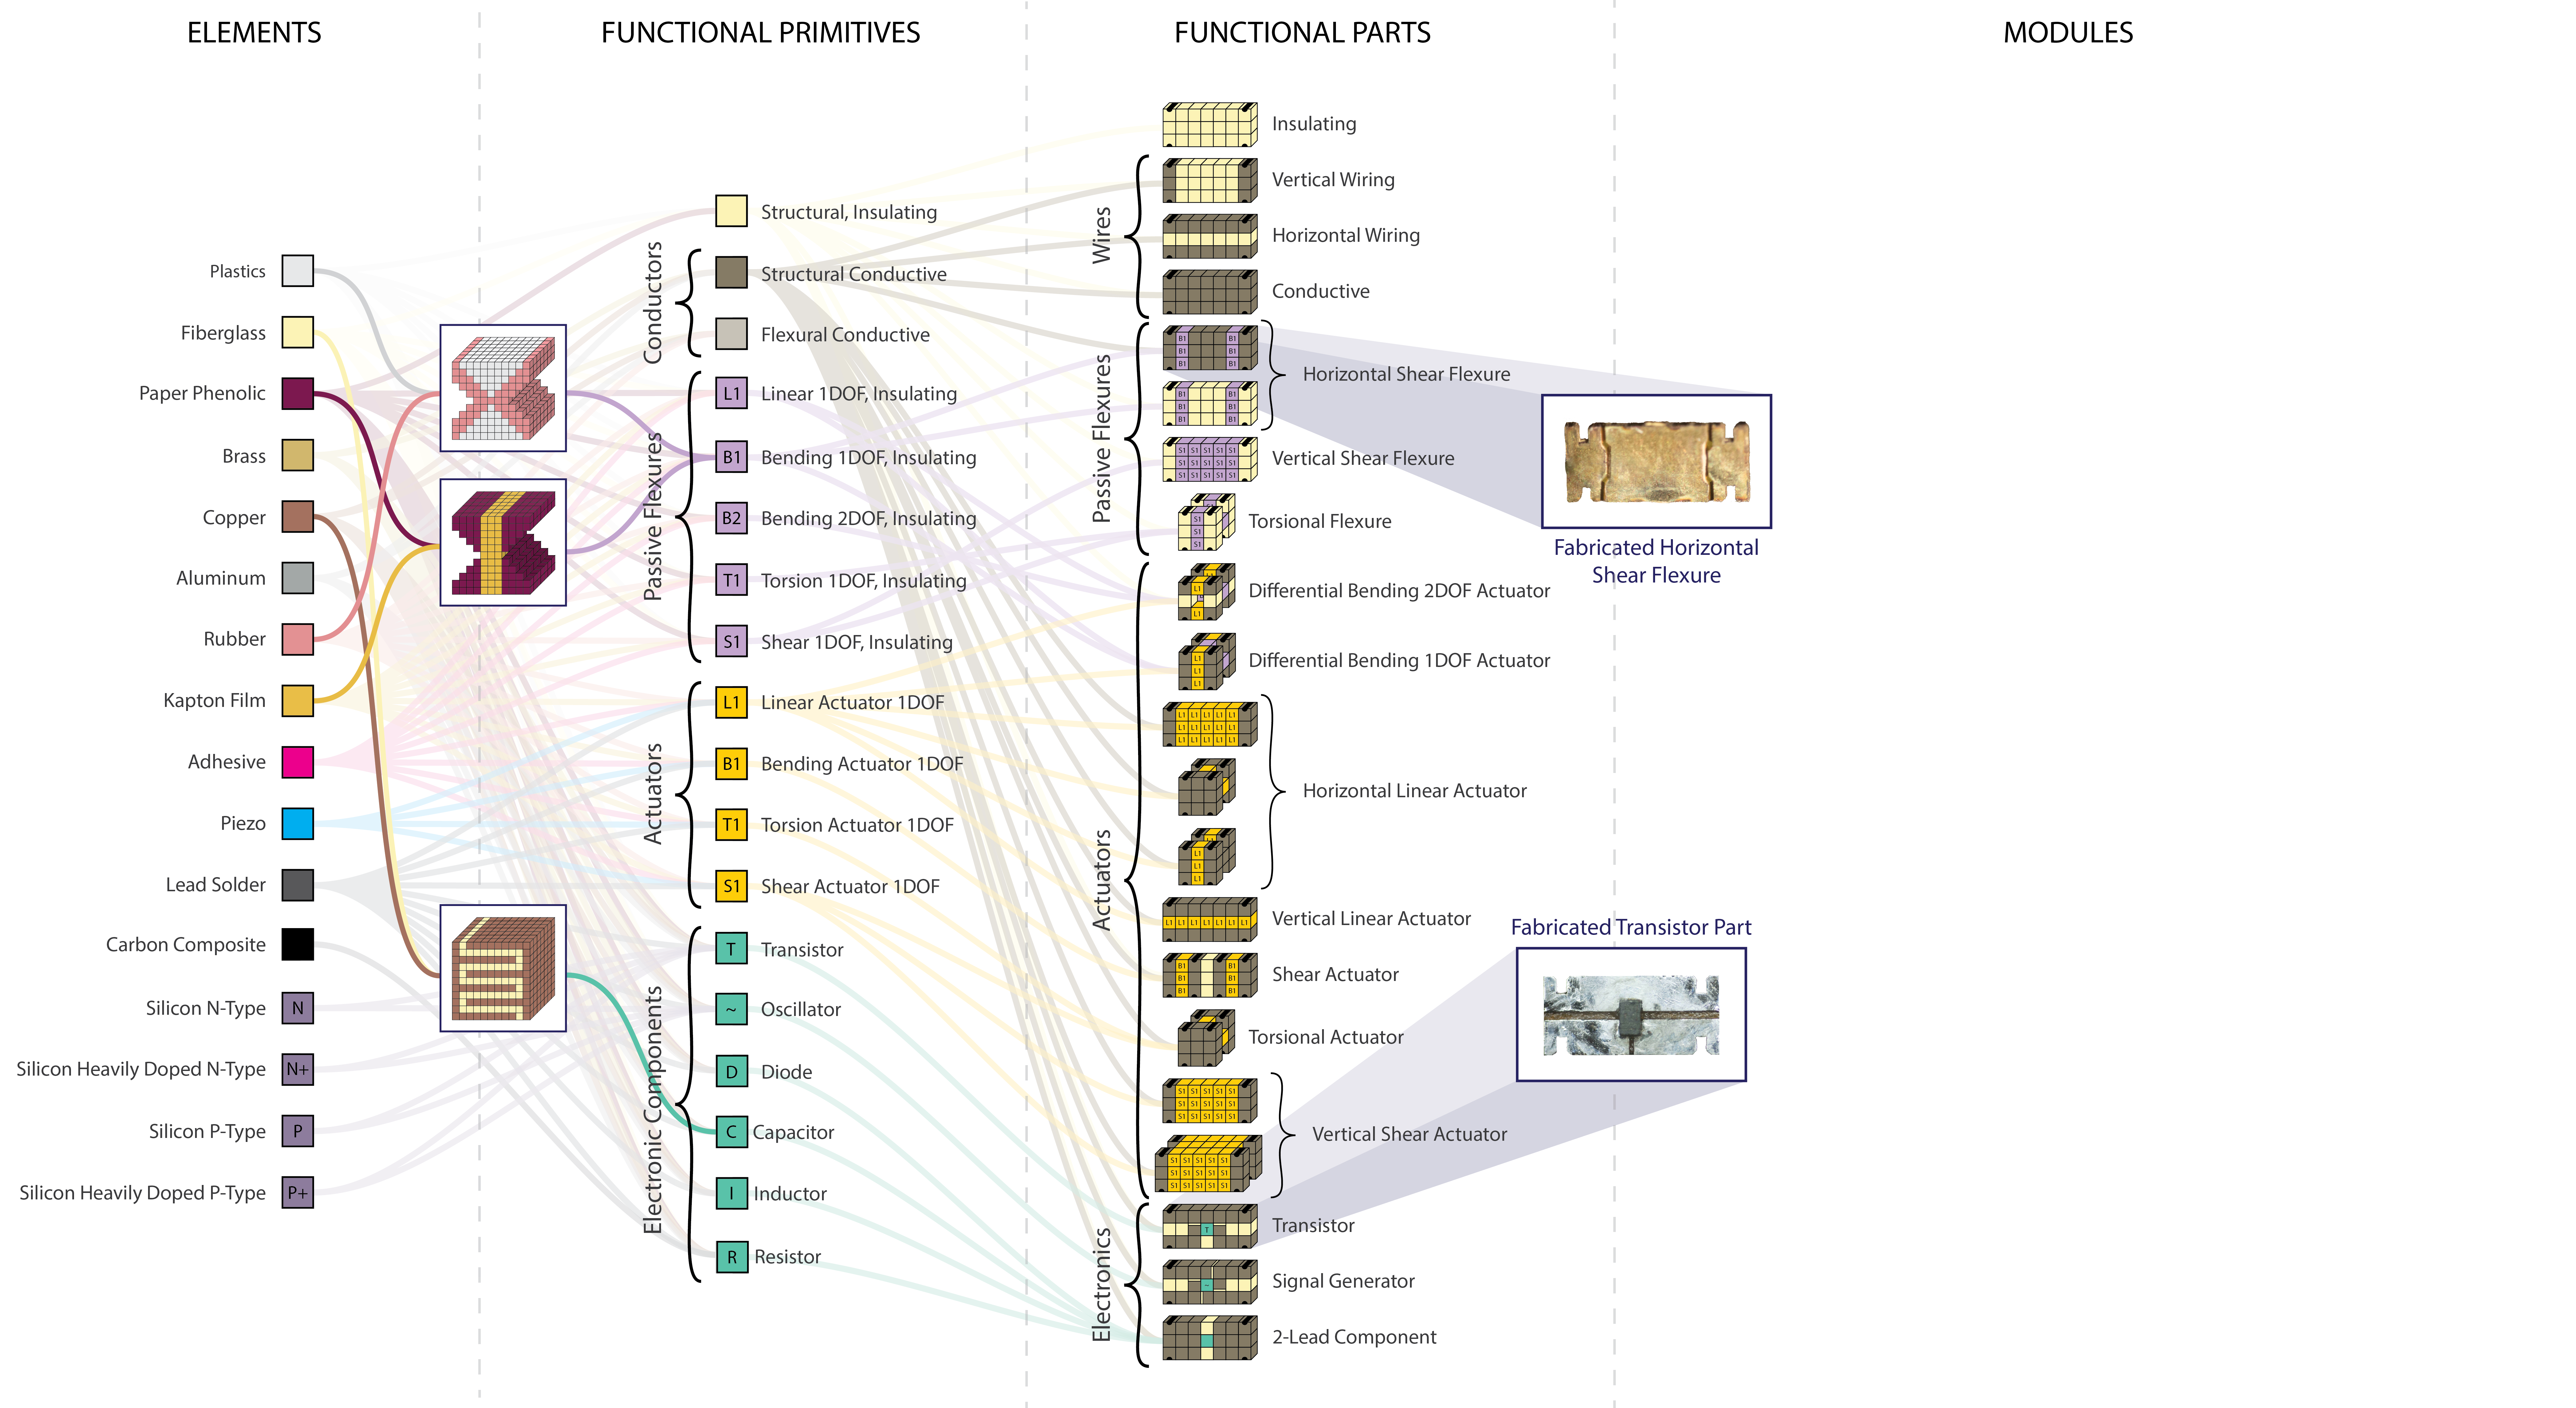
\includegraphics[width=\textwidth,height=\textheight,keepaspectratio]{FullHierarchy.png}
  \caption{Diagram of the hierarchical breakdown of robotic modules into functions and elements.  Examples of the geometric layout of elements to form functional primitives are indicated for a 1DOF bending flexure and a capacitor.  Images of fabricated functional parts are shown alongside their functional primitive decompositions.  More detailed views of the transition from elements to functional primitives and from functional primitives to functional parts are shown in Figures \ref{fig:Hierarchy-ElementsParts} and \ref{fig:Hierarchy-FunctionPrimitivesParts}.  \textit{Image Credit (for photos of fabricated functional parts): Will Langford 2016} }
  \label{fig:FullHierarchy}
\end{sidewaysfigure}

\begin{figure}
  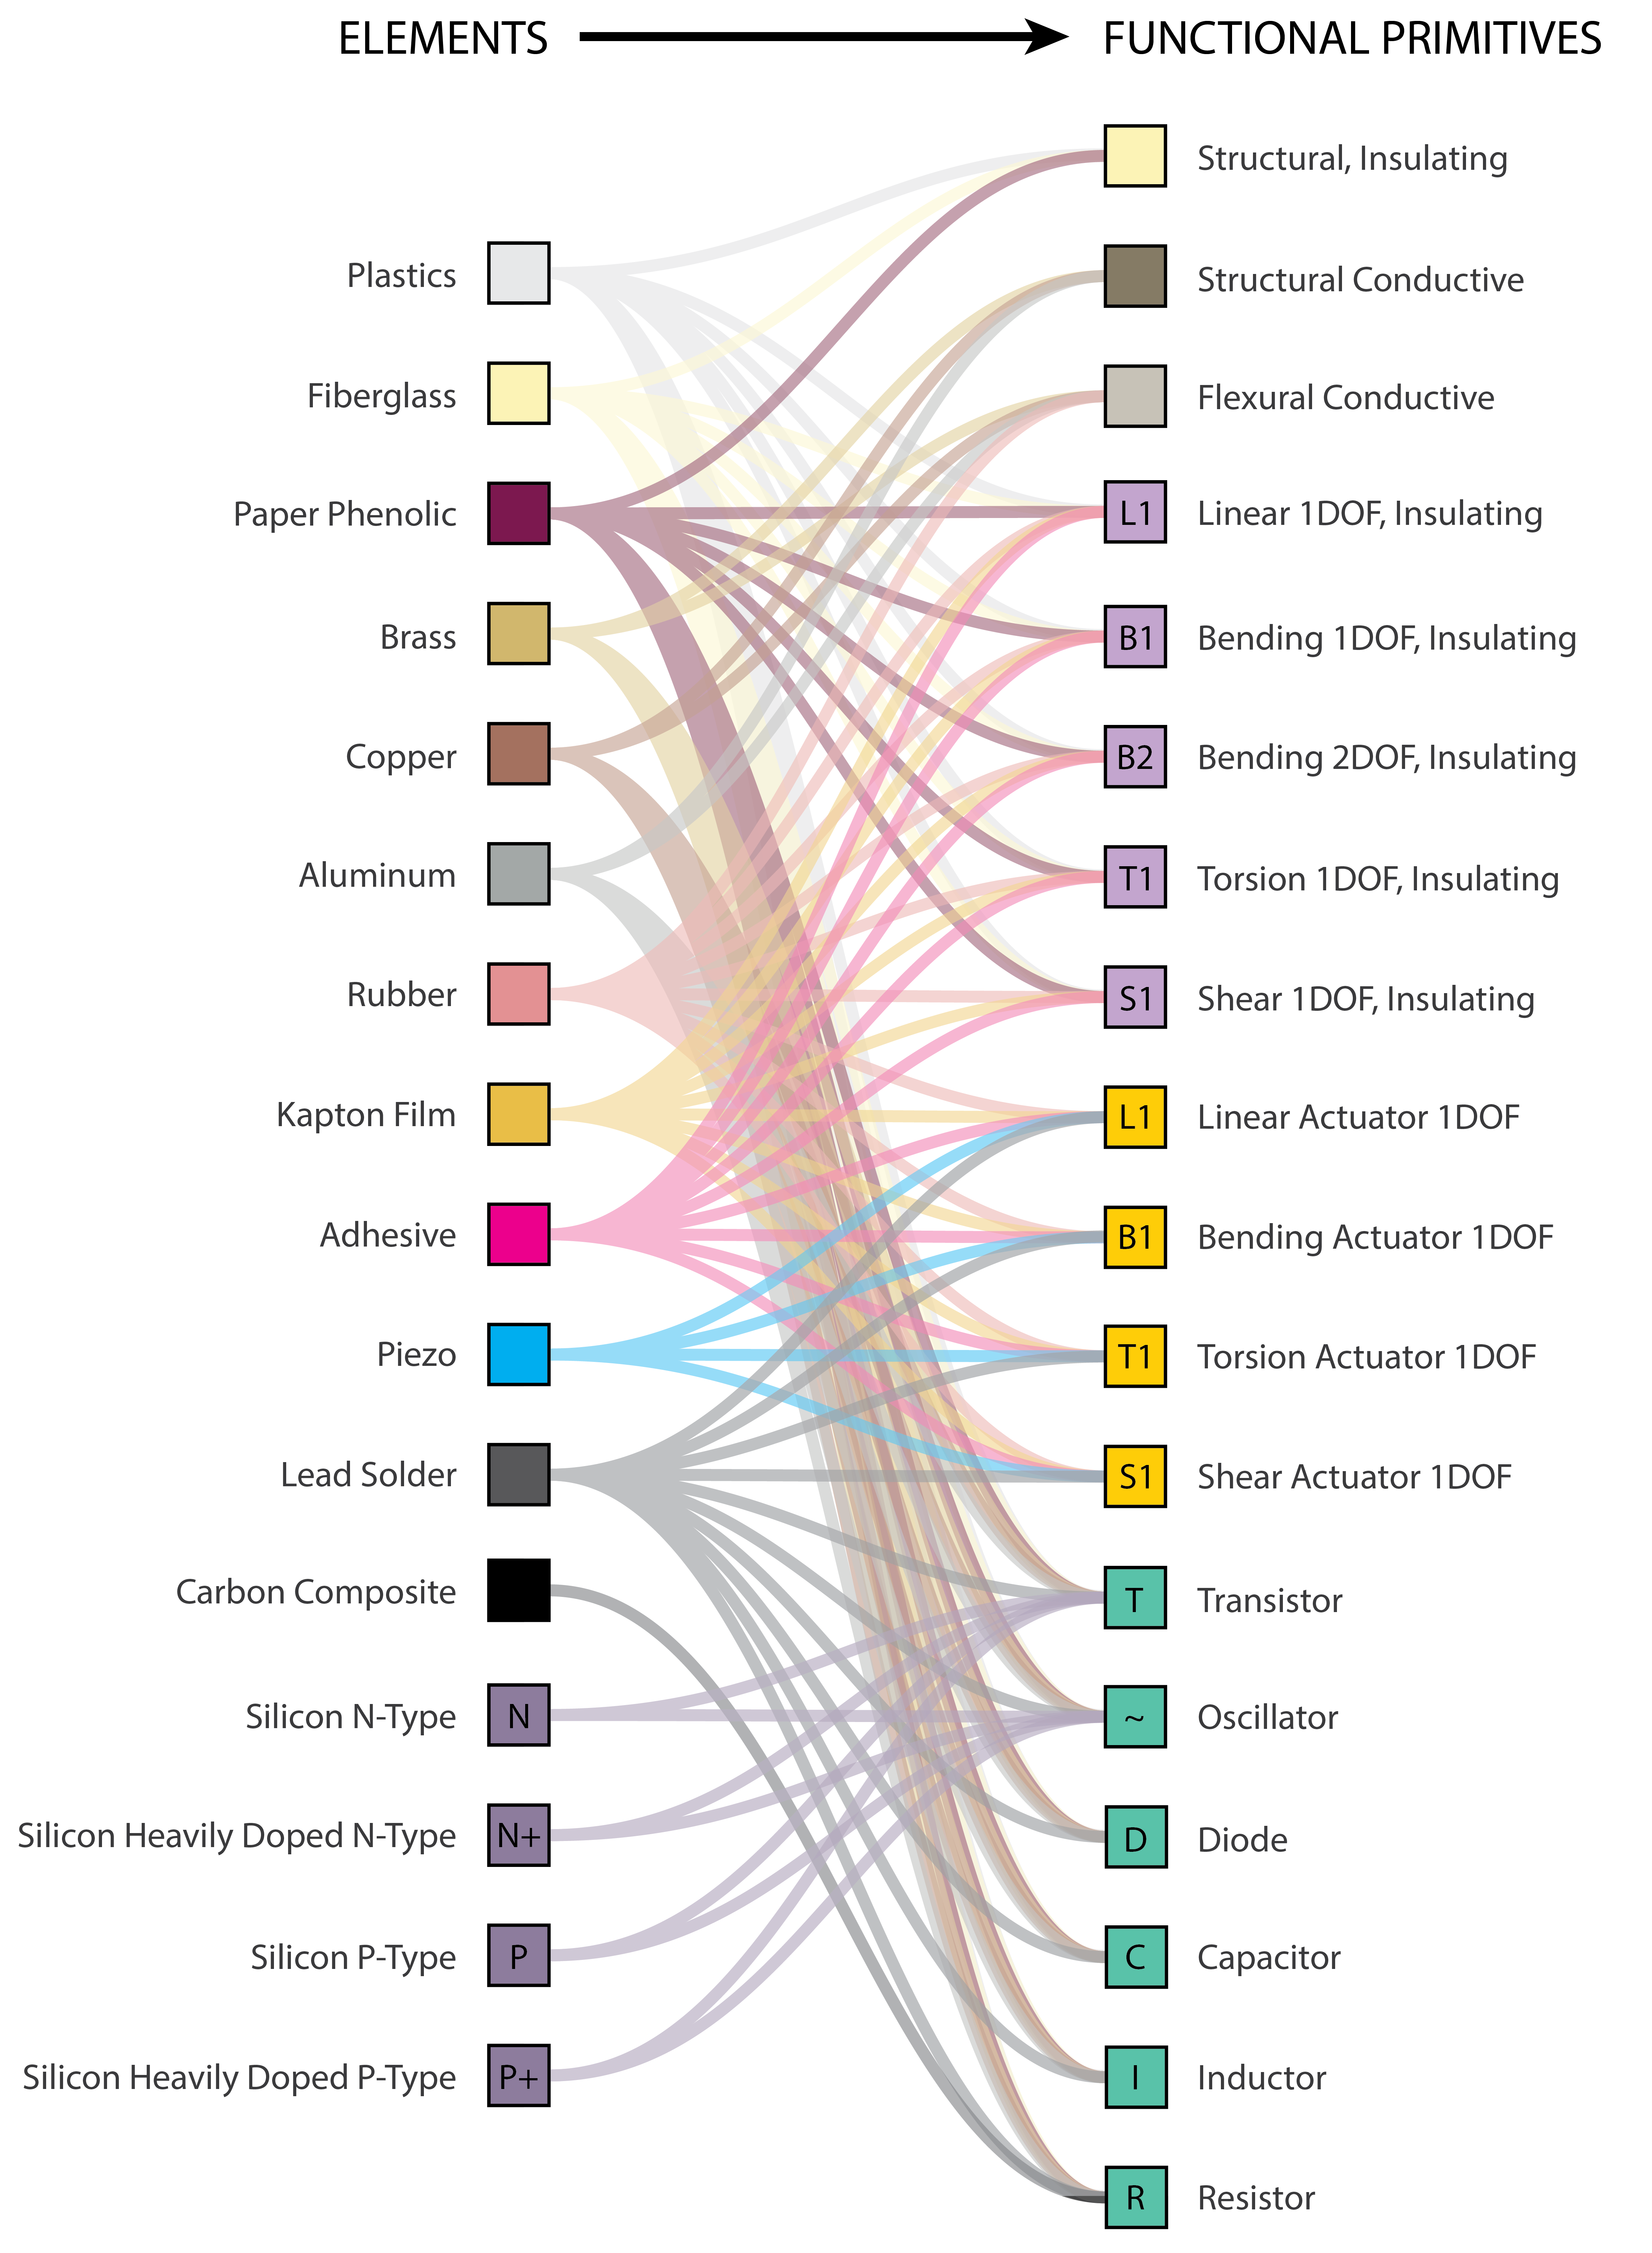
\includegraphics[width=\linewidth]{Hierarchy-ElementsParts.png}
  \caption{Detail view of Figure \ref{fig:FullHierarchy}, explaining the elemental materials that go into each functional primitive.}
  \label{fig:Hierarchy-ElementsParts}
\end{figure}

\begin{figure}
  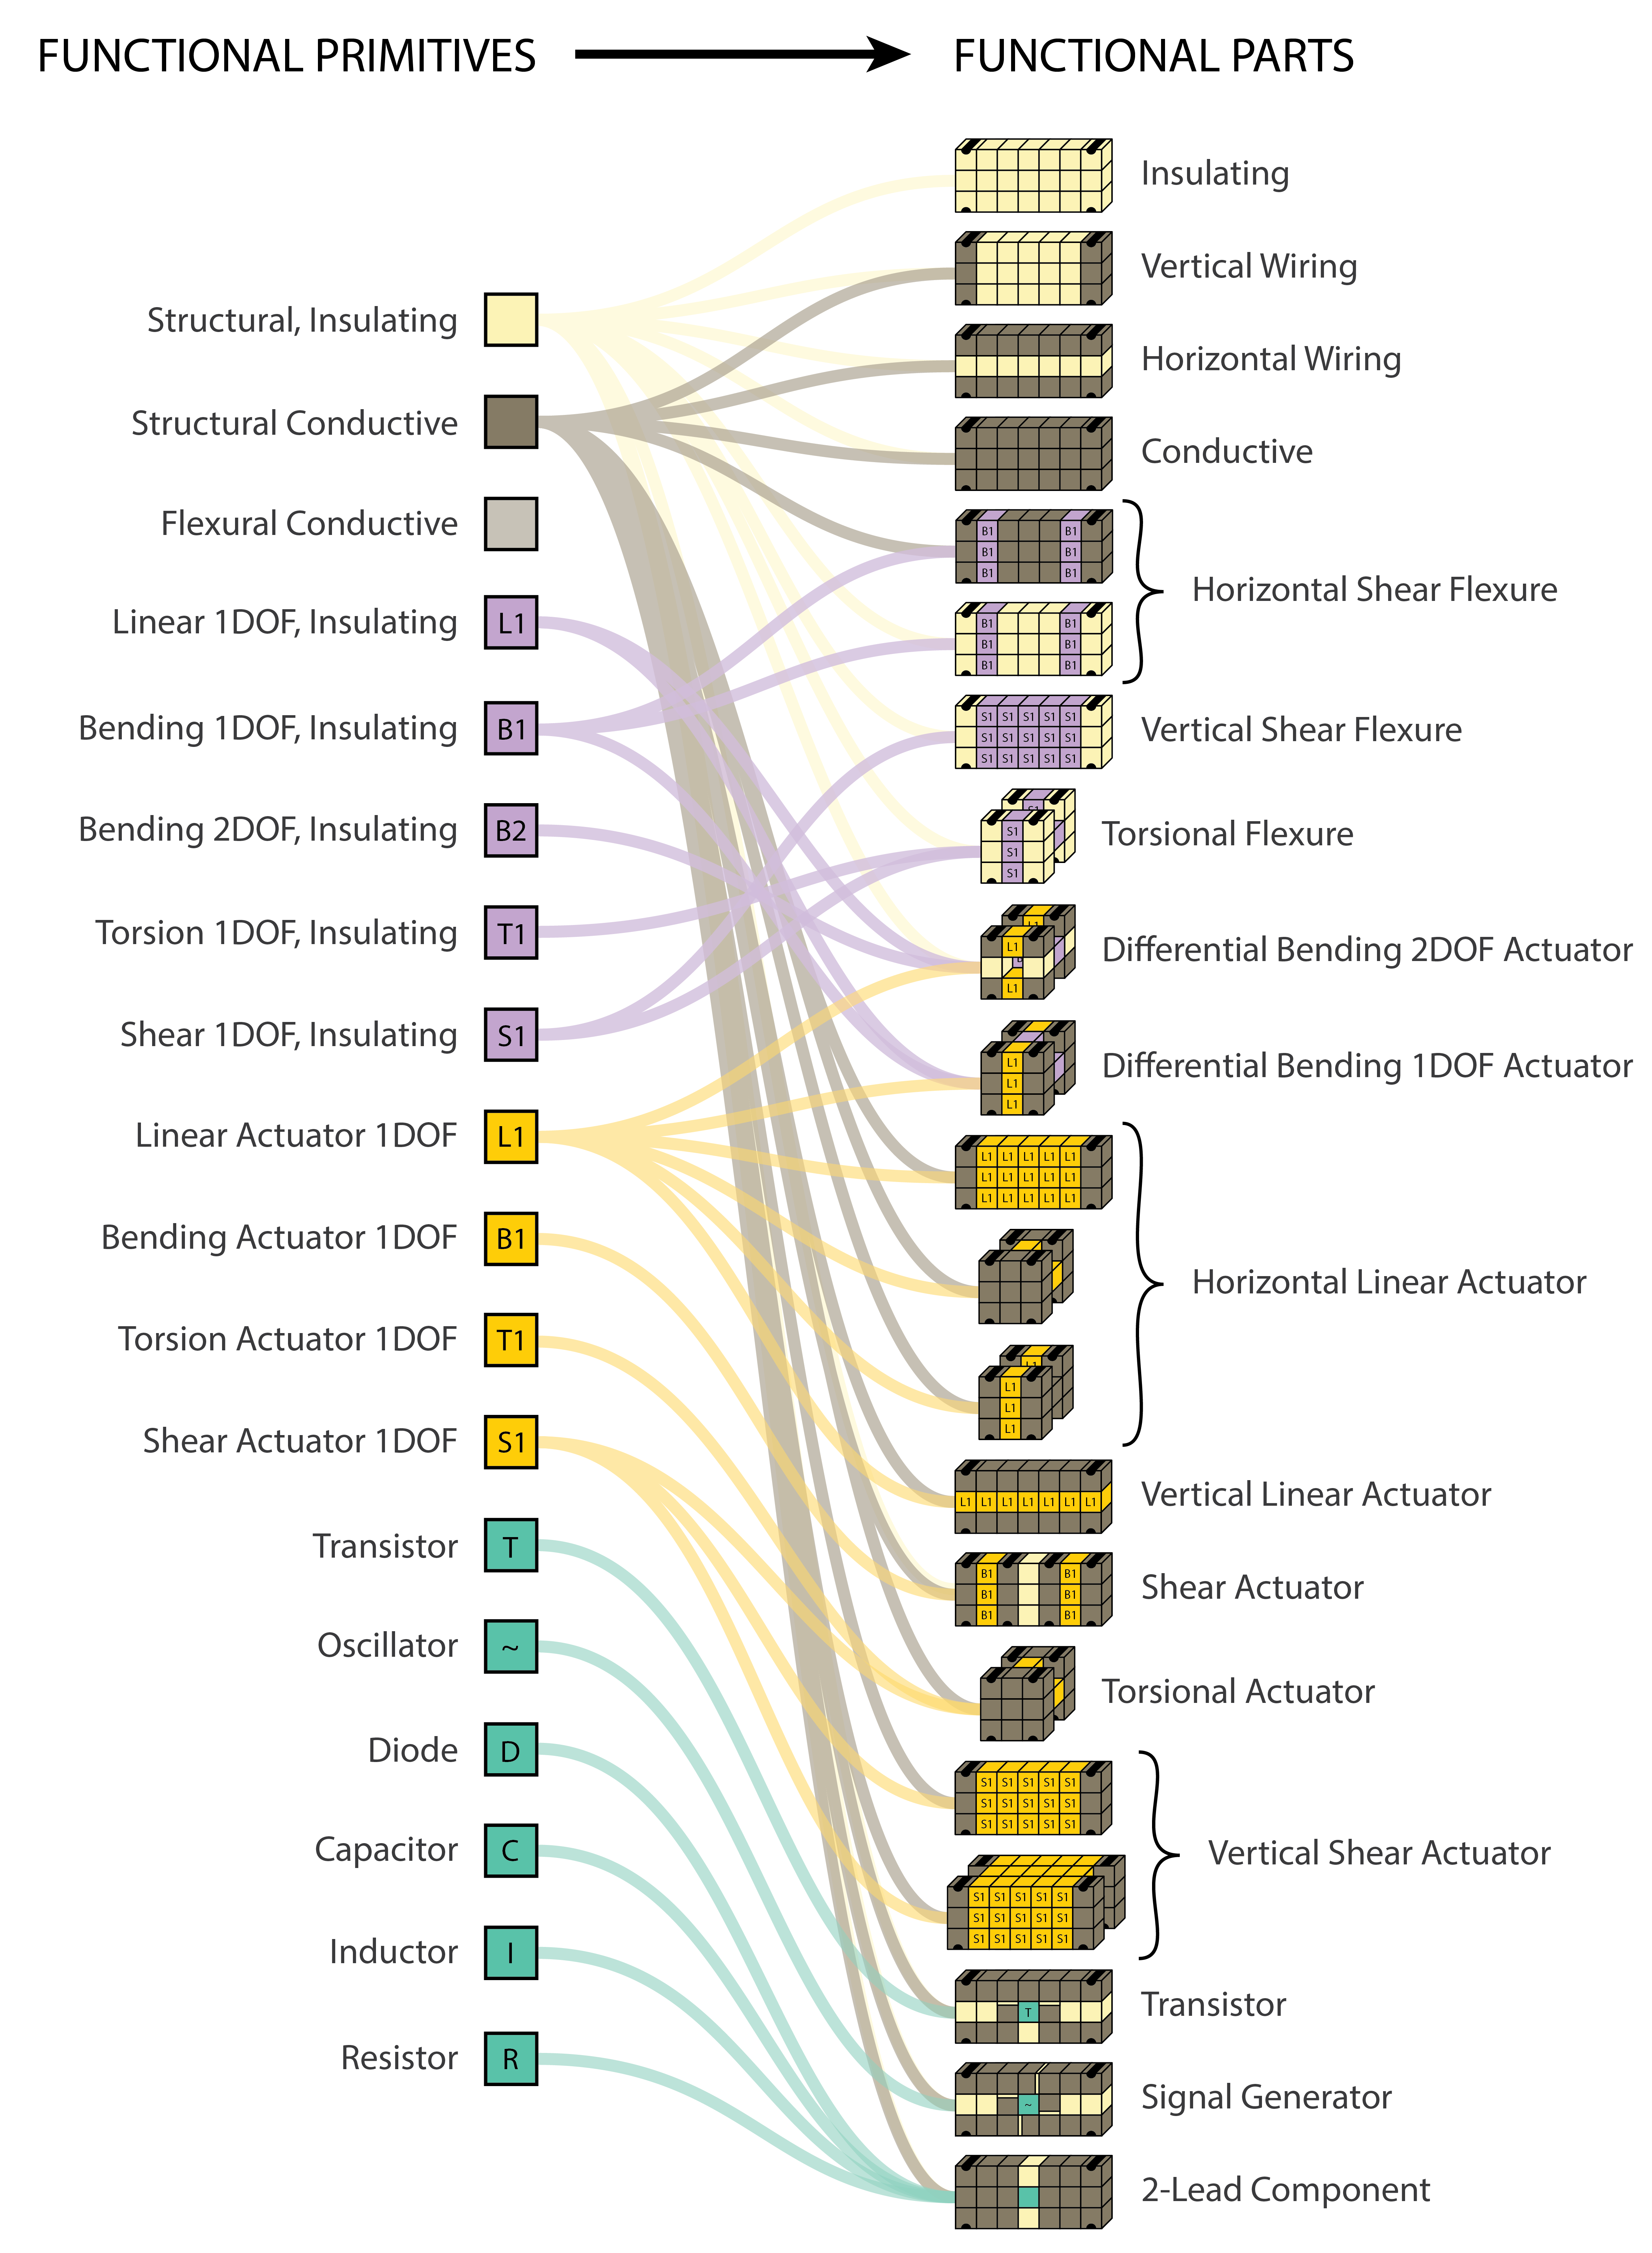
\includegraphics[width=\linewidth]{Hierarchy-FunctionPrimitivesParts.png}
  \caption{Detail view of Figure \ref{fig:FullHierarchy}, explaining the decomposition of functional parts into functional primitives.  Part-part interface of functional parts is indicated in black.}
  \label{fig:Hierarchy-FunctionPrimitivesParts}
\end{figure}

\section{Elements}\label{sec:elements}

At the lowest level, bulk materials in the form of \textit{elements} are assembled together to form multi-material assemblies.  Our notion of "element" is not an atomic element, but rather a homogenous volume of material with characteristic material properties.  A finite set of elemental types will be chosen based on desirable physical properties, cost, ease of fabrication, and compatibility with other elemental types and assembly processes.\\

For example, an aluminum element type would have the properties of being conductive, stiff, and lightweight and a rubber element type would be insulating and flexible.  Current elements types of interest are described in Figure \ref{fig:Hierarchy-ElementsParts}.  Other element types may include magnetic and magnetically permeable types, additional actuation types, and thermally conductive and insulating types.\\

Elemental components will be fabricated to a size on the order of $\sim$1-10$\mu$m\textsuperscript{3}.  Some, as yet to be determined, form of joining interface must be incorporated into the geometry of the elemental parts or applied (in the form of an adhesive) to the parts during the assembly process.  At this point in time, we envision a permanent joining strategy between elemental parts.

\section{Functions}

Assemblies of elements form \textit{functions} - larger scale part types with material properties defined by their constituent elements.  As the name suggests, functions are categorized based on higher-level interactions with neighbors, rather than their bulk material properties.\\

From a software perspective it makes sense to break down the function category into two layers: \textit{functional primitives} and \textit{functional parts}.  Functional primitives are a useful abstraction that serve as the fundamental unit for simulation of functional parts, described in more detail in Chapter \ref{chap:functionSim}.  Functional parts, on the other hand, are small motifs of functional primitives, complete with interfacing joinery, that form the basis of function-level fabrication and assembly.  This distinction is analogous to the cell/supercell delineation used for GIK parts, described in Chapter \ref{chap:CAD}.\\

Functional primitives fall into one of several functional archetypes, including n-degree-of-freedom mechanical flexures and actuators, and simple passive and active electronic components.  These archetypes are represented chromatically in Figure \ref{fig:Hierarchy-FunctionPrimitivesParts}.  The "function" of a functional primitive is determined by the 3D composition of its constituent elements, depicted in Figure \ref{fig:FullHierarchy}.  Anisotropic patterns of elemental types within a functional primitive may give it tunable anisotropic behaviors.  A more complete discussion of the diversity of mechanical and electronic part types at the function-level is given in Chapter \ref{chap:functionSim}.  In the fullness of time, the geometric composition of functional primitives from elements would be a good candidate for constrained topological optimization.\\

Functional parts are small assemblies of functional primitives, plus a joining interface.  Because functional parts are not dramatically more complex than function primitives, their behaviors are more or less the same.  A selection of potential functional parts are diagramed in Figure \ref{fig:Hierarchy-FunctionPrimitivesParts}, though that list is not meant to be exhaustive.  Examples include routing components, which pass one or several electronic signals to neighboring parts, anisotropic flexural and actuated parts, and simple passive and active electronic components.\\

Functional parts are currently fabricated using irreversible, bulk 2D processes on the order of $\sim$1mm\textsuperscript{3}.  Some form of common interface must allow for both mechanical loads and analog electronic signals to pass from one functional part to another.  At the function-level, a reversible joining interface is preferred so that reconfigurable behavior and recycling is possible.  Currently, press-fit or reversible soldered interfaces are being explored.  The first attempts at fabricating functional parts (by Will Langford) is depicted in Figure \ref{fig:FullHierarchy}.

\section{Modules}

\textit{Modules} are assemblies of function-level components, joined together to form robotic subsystems.  Modules combine electronic and mechanical functionality to achieve singular, high-level robotic tasks.  Modules will communicate with each other through an abstracted, digital interface.  Each module will own its own microprocessing unit that coordinates its function-level actuators and other active components.  This way, the low-level description of the structure within a module remains internal to the module itself.\\

Examples of modules include end effectors like grippers, clamping mechanisms, and sensors, actuation/locomotion systems, energy storage and generation, and large memory or programmable logic banks.  Joining interfaces between modules will allow mechanical forces, power, and a few digital signals to pass from one module to the next.  As with functions, modules should be reversibly joined.  The interface between modules may consist of many parallel function-level interfaces, or a bulk, module-level interface.\\

Modules will be built on the order of $\sim$1cm\textsuperscript{3}.  Though modules may use mechanical compliance at the function-level to increase their internal degrees of freedom, at larger scales modules act as rigid bodies with internal motion.  That is, internal mechanical compliance within a module does not propagate to interactions with neighboring modules.%This idea follows from a model of how traditional solid-bodied rotary and linear actuators are viewed within a larger robotic structure.

\section{Complexes}

Assemblies of modules form \textit{complexes}, self-contained robotic systems that coordinate their own sensing, memory, logic, power, and/or actuation.  Though a module should be sophisticated enough to control its own actuators, a complex ties together input and output modules to produce interactive behavior.  Instructions may be fed to complexes through their environment in order to direct large scale processes involving many complexes in parallel.  In this case, complexes will need to maintain electronic contact with environmental signaling wires.  Initial complex design may also depend on power sourced through the complex's environment.\\

A complex could be a single, locomoting robot or manipulator, or an active, environmental system that performs sensing, actuation, or logical tasks across space.  Complexes will interact with function-level and module-level feedstock to accomplish assembly tasks.  Many complexes will work together to shuttle these feedstock around space and pick and place them in a directed, programmable fashion.\\

Complexes will be comprised of $\sim$10-100 individual modules, spanning length scales on the order of tens of cm to m.  Complexes should be considered independent, self-contained units with quantized motions.  The interface between complexes is governed by end effector modules that the complex owns.

\section{Systems of Complexes}

Many complexes of various forms and functions may work together at a \textit{system}-level to accomplish large scale tasks.  Additional layers of hierarchy could be introduced to manage these systems.  For now, a systems-level discussion is beyond the scope of this work.

\section{Design Hierarchy in Biology}\label{sec:biologyHierarchy}

\begin{sidewaysfigure}
  \includegraphics[width=\textwidth,height=\textheight,keepaspectratio]{ProteinHierarchy.png}
  \caption{Hierarchical breakdown of protein complexes (complexes) into proteins (modules), amino acids (functions), and atoms (elements).  3D renderings of protein complexes and subunits were made in \href{https://www.pymol.org/}{Pymol} using data from the RCSB Protein Data Bank  \cite{UCSD/SDSC}.}
  \label{fig:ProteinHierarchy}
\end{sidewaysfigure}


Currently, the only known physical example of a self-replicating system is the biology that has evolved on Earth.  The primary drivers of biological self-replication are protein machinery (called "protein complexes") built primarily from a small set of amino acid building blocks.\\

The construction of protein complexes takes place in a hierarchical fashion.  Figure \ref{fig:ProteinHierarchy} describes the hierarchical breakdown of protein complexes in terms of the four levels of hierarchy established earlier in this chapter; protein complexes (complex-level objects) are decomposed into proteins (modules), then into amino acids (functions), and finally into atoms (elements).  The similarity of some of the biological nomenclature to our own hierarchical nomenclature is due to the fact that it was derived from the biological model.
%This hierarchical breakdown is slightly different from the primary/secondary/tertiary/quaternary structures often used to discuss the levels of protein description.  

\subsection{Elements, Functional Groups, and Functions}

At the most fundamental level, biological structures are composed of atoms of various elemental types.  On Earth, biological molecules are made primarily from combinations of carbon, hydrogen, nitrogen, oxygen, phosphorus, and sulfur (CHNOPS).\\

Each element's unique position on the periodic table dictates its physical properties, which have implications in higher-level structures formed from the element.  These properties include mass, the number of covalent bonds it can form, the number of paired electrons it contains in its outermost electron shell, the polarization of the bonds and molecules it forms with other elements, and the stability of its bonds in various environments.\\

Certain motifs of covalently bonded atoms form \textit{functional groups} within molecules.  Functional groups determine the ability of a molecule to undergo various archetypal reactions (addition, substitution, elimination, etc) with itself or other molecules.  A subset of the important functional groups found in biochemistry are indicated in Figure \ref{fig:ProteinHierarchy}.  "R" indicates an arbitrary side-chain, where the functional group connects to the rest of the molecule.\\

%In organic chemistry, the identification of functional groups allow us to abstract the interactions between molecules based on to predict how they will react in certain conditions.


\begin{figure}
  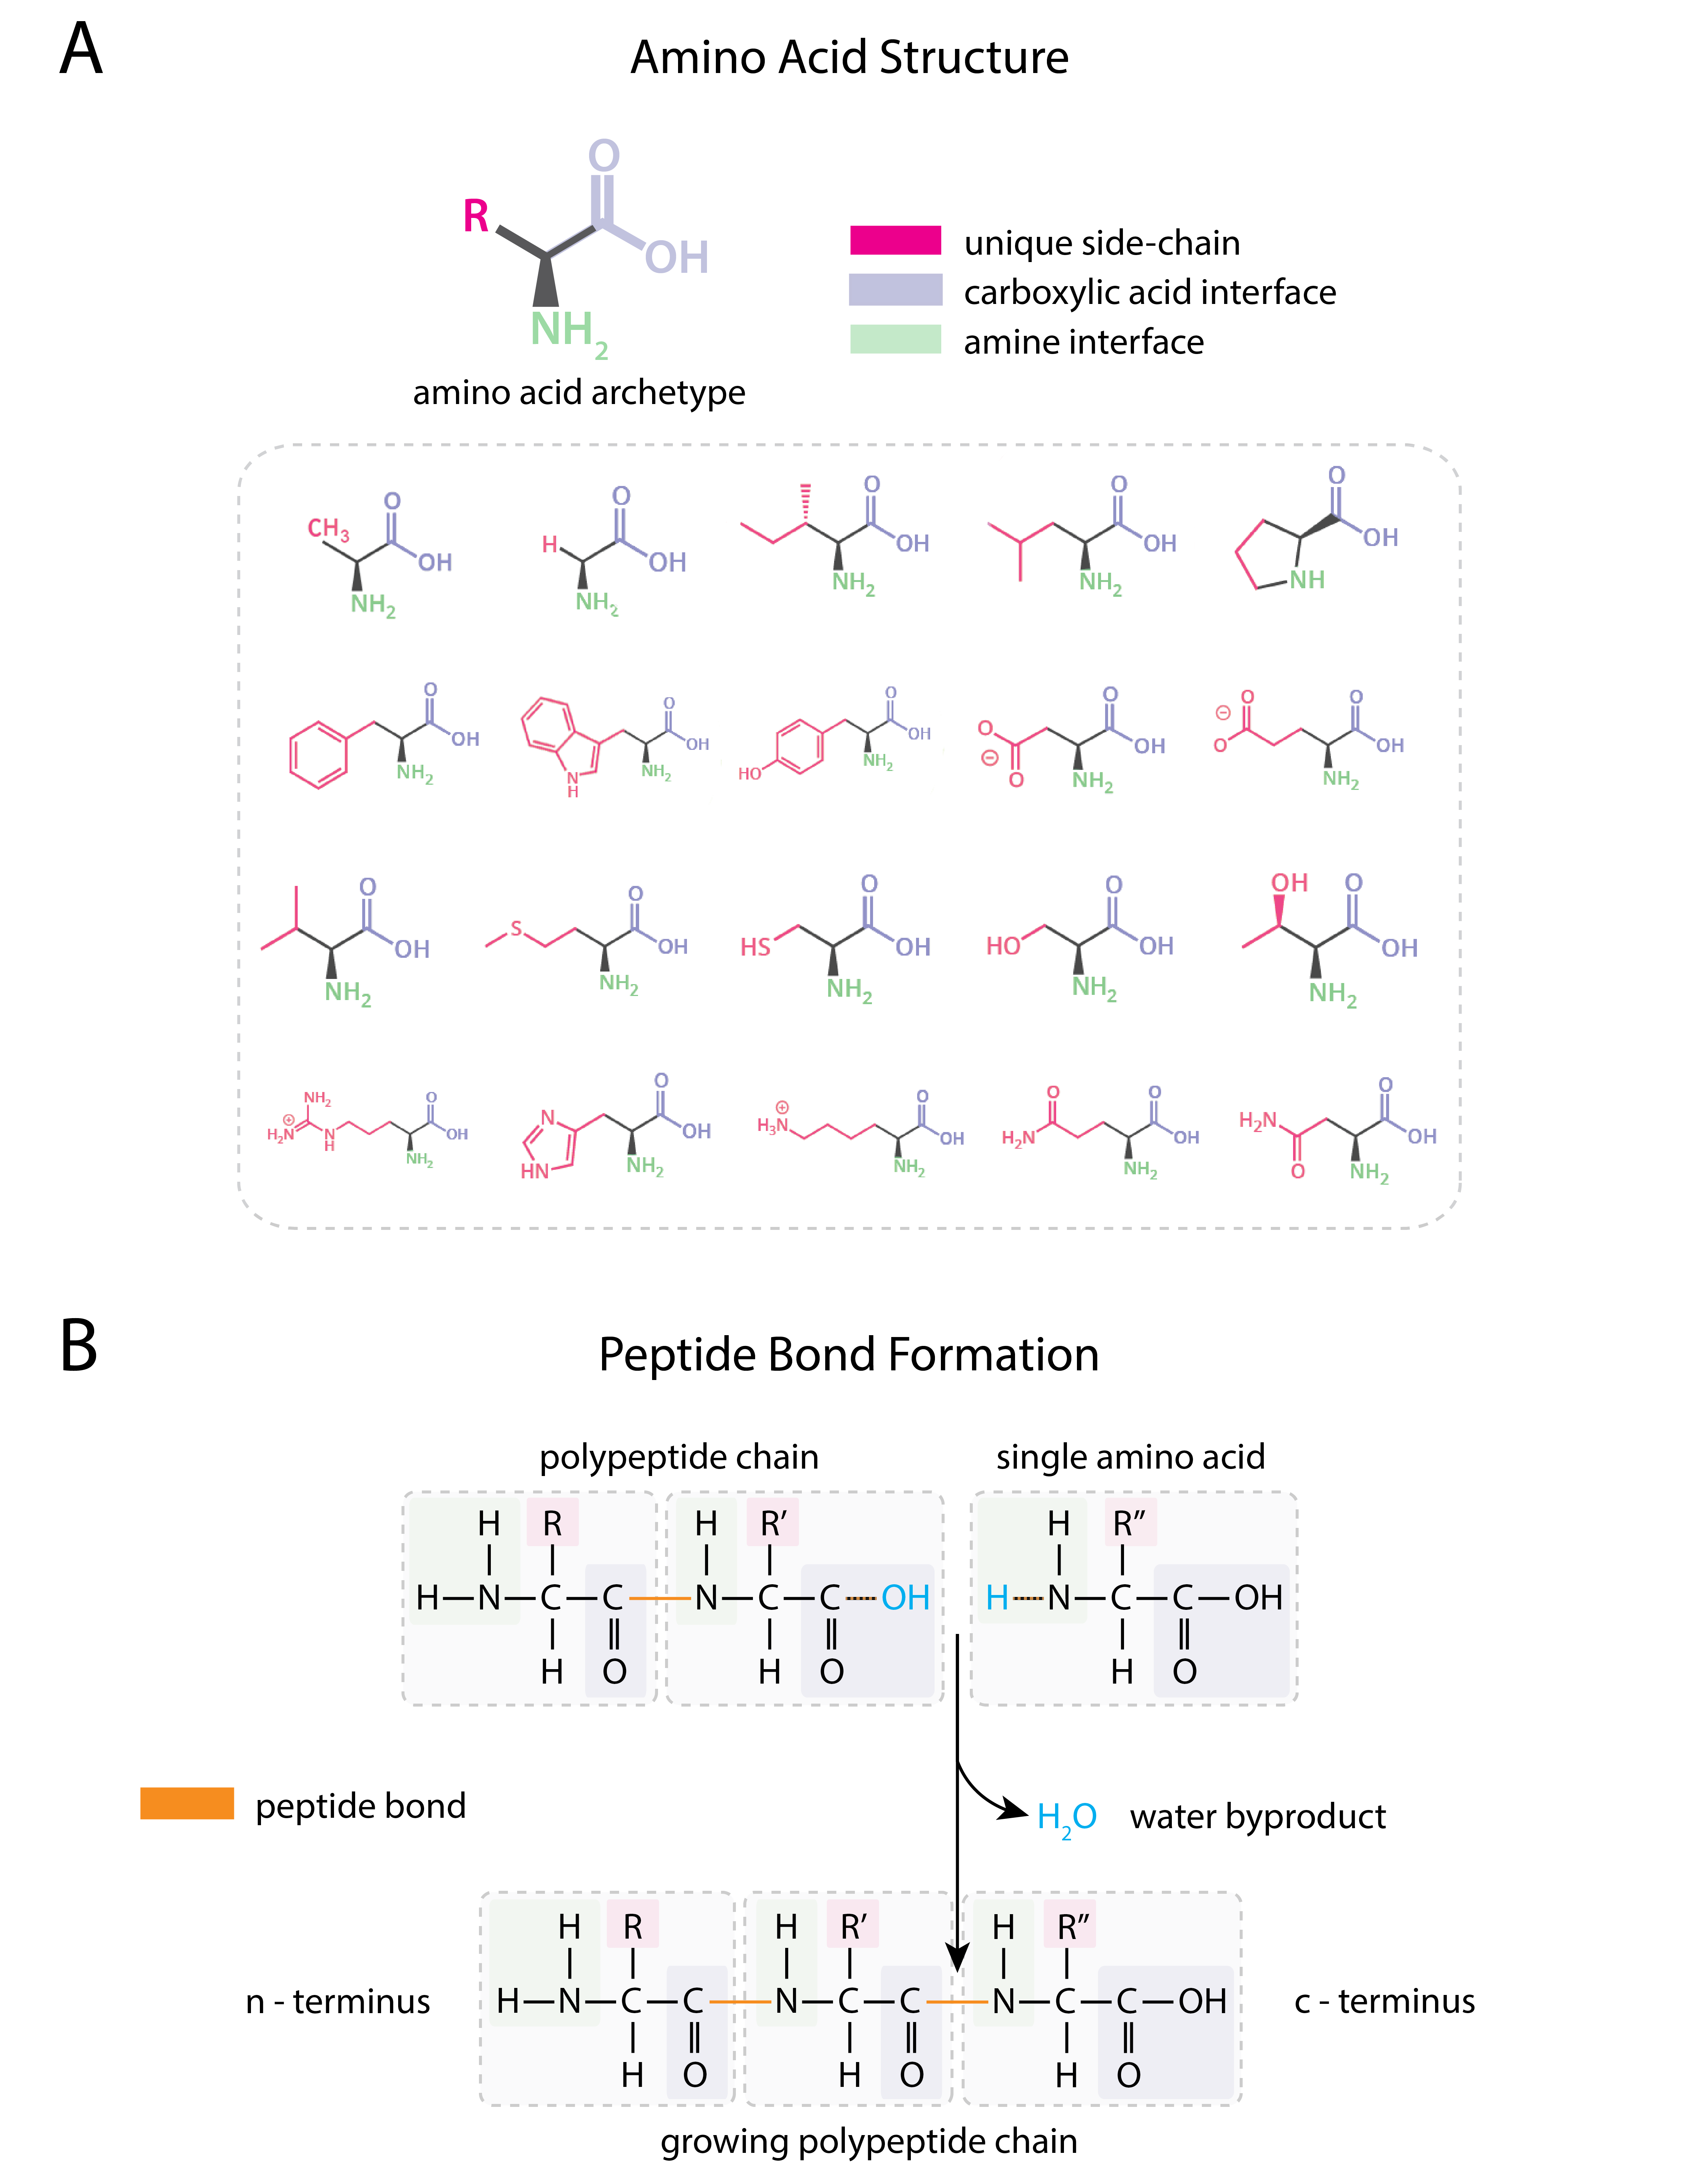
\includegraphics[width=\textwidth]{AminosInterface.png}
  \caption{(A) Decomposition of amino acids into carboxylic acid and amine interfaces and unique side-chain. (B) Formation of peptide bond at c-terminus (carboxylic acid group) of polypeptide chain with the n-terminus (amine group) of an amino acid. One molecule of water is produced as a byproduct of the peptide bonding reaction.  R, R', and R'' represent arbitrary amino acid side-chains.  Peptide bonds bolded.}
  \label{fig:AminosInterface}
\end{figure}

\textit{Amino acids} are molecules which contain several functional groups.  As indicated in Figure \ref{fig:AminosInterface}A all amino acids contain a carboxylic acid (COOH) and an amine group (NH\textsubscript{2} or NRH).  The purpose of these groups is to form the interface between amino acids in a polypeptide chain.  Amino acids are attached to each other through a covalent bond, called a "peptide bond", with a single molecule of water created as a byproduct of each bonding event\ref{fig:AminosInterface}B.\\

The remainder of the amino acid molecule (indicated by "R" in the amino acid archetype in Figure \ref{fig:AminosInterface}A, we'll call it "\textit{the} side-chain") determines its unique properties.  Each type of amino acid has a different side-chain, which may consist of one or more distinct functional groups.  Amino acids are characterized according to their side-chains in several ways; one grouping is shown in Figure \ref{fig:ProteinHierarchy}, with amino acids described by size, polarity, nucleophilicity, the presence of aromatic rings, acidity or basicity, and the presence of amide groups.\\

 \subsection{Modules and Complexes}

Polypeptide chains typically consisting of hundreds of amino acids fold to form three dimensional \textit{proteins}.  Hydrogen bonding and other non-covalent interactions between amino acid side-chains, along with external effects, determine the three dimensional structure of the protein.  At the protein's active site, amino acid sidechains interact with molecules in the environment.  Sometimes, these interactions result in global deformations of the protein's three dimensional structure, called "conformational changes".\\

Multiple proteins join together through non-covalent interactions to form a \textit{protein complex}.  A protein within a complex is usually referred to as a subunit.  Protein complexes sometimes contain contain many identical subunits.

\subsection{Insights}

The main take-away from the biological model is proof of principle.  Biology demonstrates how a small basis set of simple, functional feedstock can be reversibly assembled to create more complex structures and mechanisms - ultimately, self-replicating systems.  It should be noted, however, that analogies between biological systems and our proposed assembly system are limited due primarily to differences in scale (and therefore, different types of dominant physics), rates of interactions between parts, and mechanism of interaction between parts.

\subsubsection{Scaling}

In the biological example, each level of hierarchy introduces a factor of about 10x in scaling.  The atoms that compose the lowest level of hierarchy have covalent diameters ranging from 50-200pm  \cite{Slater1993}.  Amino acid diameters can be roughly calculated from atomic radii and three-dimensional structure to a range of 0.42-1.2nm  \cite{Pool2003}.  The average protein length across prokaryotes and eukaryotes is about 200-400 amino acids, with a mass of about 20-40kDa  \cite{Brocchieri2005}.  Assuming a simple spherical shape, this mass translates to a typical protein diameter of about 3-4nm  \cite{Erickson2009}.  Known protein complexes are comprised of two to several hundred protein monomers with typical complex diameters ranging from about 8-100nm  \cite{Yang2010a}.

%Beyond these first four hierarchical levels, higher systems...
%Assembly within is not carried out by a single protein complex, but rather, by the coordinated efforts of several complexes.
%Beyond protein complexes, more levels of hierarchy exist within biological organisms to carry out systems-level tasks.  Protein complexes can be grouped according to the chemical pathways they interact with within a cell, by the organelles they belong to                                                                                                                                                                                                 
%
%Organelles are organized within cells, cells within tissues, tissues within organs, organs within even higher level systems, and ultimately these systems come together in one complete organism.

%Other evidence points to an expansion of proteinogenic amino acids over time.\\
%
%An amino acid is defined as a molecule with an amine group, a carboxylic acid group, and a side-chain.  Only 23 amino acids are proteinogenic, meaning they are used to build proteins, however non-proteinogenic amino acids are found elsewhere in the cell.  As of 1983 there were about 500 known naturally occurring amino acids.  Some of these compounds form intermediates in biochemical pathways, including pathways to synthesize proteinogenic amino acids \cite{Wagner1983}.  Many of them are toxic to humans.\\
%
%why not more?\\
%
%number of protiens\\
%number of complexes - design modularity, reusability of modules

\subsubsection{Design and Fabrication}

%In biology, protein polymerization happens in one dimension with subsequent folding into three dimensions; we must design our joining interface to accommodate something analogous to "polymerization" in three dimensions.\\

%Peptide bonding is a reversible process that occurs in both directions in a cell.  A condensation reaction removes a molecule of water and covalently bonds amino acids (Figure \ref{fig:AminosInterface}B).   A hydrolysis reaction reverses this process, using a molecule of water to break the peptide bond.  In some sense we can think of the water molecule as a type of locking mechanism in a reversible, pinned interface.  The enzymes that catalyze the forward and backward reactions are like the machinery needed to lock and unlock the pin, or to solder and de-solder a reversibly soldered joint.\\

Despite the striking complexity gap between biological systems and the nutrients required to sustain them, we should not think of biological systems as making everything they need "from scratch".  The raw material feedstock of biology contains some inherent structure and function.  Humans only synthesize 11 of the 20 standard amino acids; we must absorb the remaining "essential" amino acids from food.  Even considering organisms that do make all their amino acids, biological synthesis pathways begin with reactive precursors rather than exclusively elemental forms of atomic feedstock \cite{Stryer1988}.  Disassembly takes place with similar granularity.  Cells break down proteins into amino acids in a process called "proteolysis"; the freed amino acids are then used to construct new proteins.  Typically, amino acids are not metabolized into smaller components unless the cell has an excess of amino acids or lacks the glucose needed meet its energy needs \cite{Stryer1988}.\\

%We're mirroring the basic design of amino acids in the function-level parts of our proposed assembly system.  
Following this biological model, our lowest-level, reversibly assembled parts should also have some built-in structure and function.  As described in Figure \ref{fig:AminosInterface}A, we can think of an amino acid as being composed of a unique, functional side-chain and a standard, reversible interface.  The functional parts depicted in Figure \ref{fig:Hierarchy-FunctionPrimitivesParts} share this same basic structure.  I hesitate to draw the same analogy with the element-level, bulk material parts described in Section \ref{sec:elements}.  Differences in interaction properties (elasticity, fracture susceptibility) and available manufacturing processes for each of the elemental types listed in Figure \ref{fig:Hierarchy-ElementsParts} pose significant challenges to a universal, reversible joining interface between single-material parts.  \\

If we designate functional parts as the lowest-level reversibly assembled parts in our assembly system, interfaces between elements could include permanent adhesives or other chemical bonding techniques.   Functional parts could be produced in large-scale, batch processes without a disassembly strategy in mind.

%\subsubsection{Combinatorics}

%This feedstock should be built from an even smaller set of elemental types.\\
%
%A major design consideration in our proposed assembly system is the number of part types needed at the element and function-levels to build useful higher-level modules and complexes.  In biology, this parameter has fluctuated over time, suggesting that the optimum number may be greater than the absolute minimum requirements for self-replication.  A widely accepted hypothesis of the origin of life is the "RNA world", a time before DNA and proteins when RNA was used both for information storage and catalytic behaviors.  Over time, proteins superseded RNA as the primary catalytic and structural component of life.  Current thought suggests that because proteins are made from 20 building blocks rather than just 4, they formed more versatile structures which were better suited for mechanistic tasks \cite{Alberts2002}.  Some artifacts from the RNA world persist today: several RNA-based enzymes, called "ribozymes" carry out tasks within the cell, and many protein complexes, included the ribosome, are made from both protein and RNA subunits.

%Functions do not need to be disassembled into element-level components in our engineered system.    
\section{Design Hierarchy in Conway's Game of Life}\label{sec:conwayHierarchy}

In the 1940's Von Neumann began studying the requirements for self-replication and evolvability in artificial, CA worlds  \cite{Neumann1966}.  One such world that has gained widespread notoriety is Conway's Game of Life ("Life").  Since its inception in 1970, Life has developed a cult following of researchers, engineers, and hobbyists, pushing each other to construct increasingly elaborate "machines" from pixels on a screen.  These investigations have resulted in a lengthy taxonomy of motifs, reactions, mechanisms, and complex engineered systems within Life.  Some notable accomplishments include Gemini (an oblique spaceship encoded by a long glider tape) \cite{Wade2010}, the Linear Propagator (a self-replicating machine) \cite{Greene2013}, a universally extensible Turing Machine  \cite{Rendell2000}, the Minsky Register Machine (a finite universal computer) \cite{Chapman2002}, and the OTCA Metapixel (a structure that behaves like a large-scale Life pixel) \cite{Due2006}.\\

The analogies between machines in Life and our proposed assembly system are limited, due to the fact that Life is inherently non-physical; it violates basic conservation principals, has no notion of cell joining, and is based on highly abstracted interactions.  However, it provides an example of how humans can engineer non-trivial self-replication from extremely simple building blocks.  A proof of the existence of self-replicating patterns in Life was first published by Conway, Berekamp, and Guy in 1982 \cite{Berekamp1982}, and several decades later the first implementations of replicators began emerging on online Life forums \cite{Greene2013a}.  This work argues that the basic requirements for self-replication - universal computation and universal construction - are not only \textit{not} unique to biology, but are, in fact, quite prevalent in virtual and physical systems.  An excellent analysis of Conway's existence proof, as well as an introduction to important concepts in Life can be found in \textit{The Recursive Universe} by William Poundstone \cite{Poundstone1985}.\\

\begin{figure}
  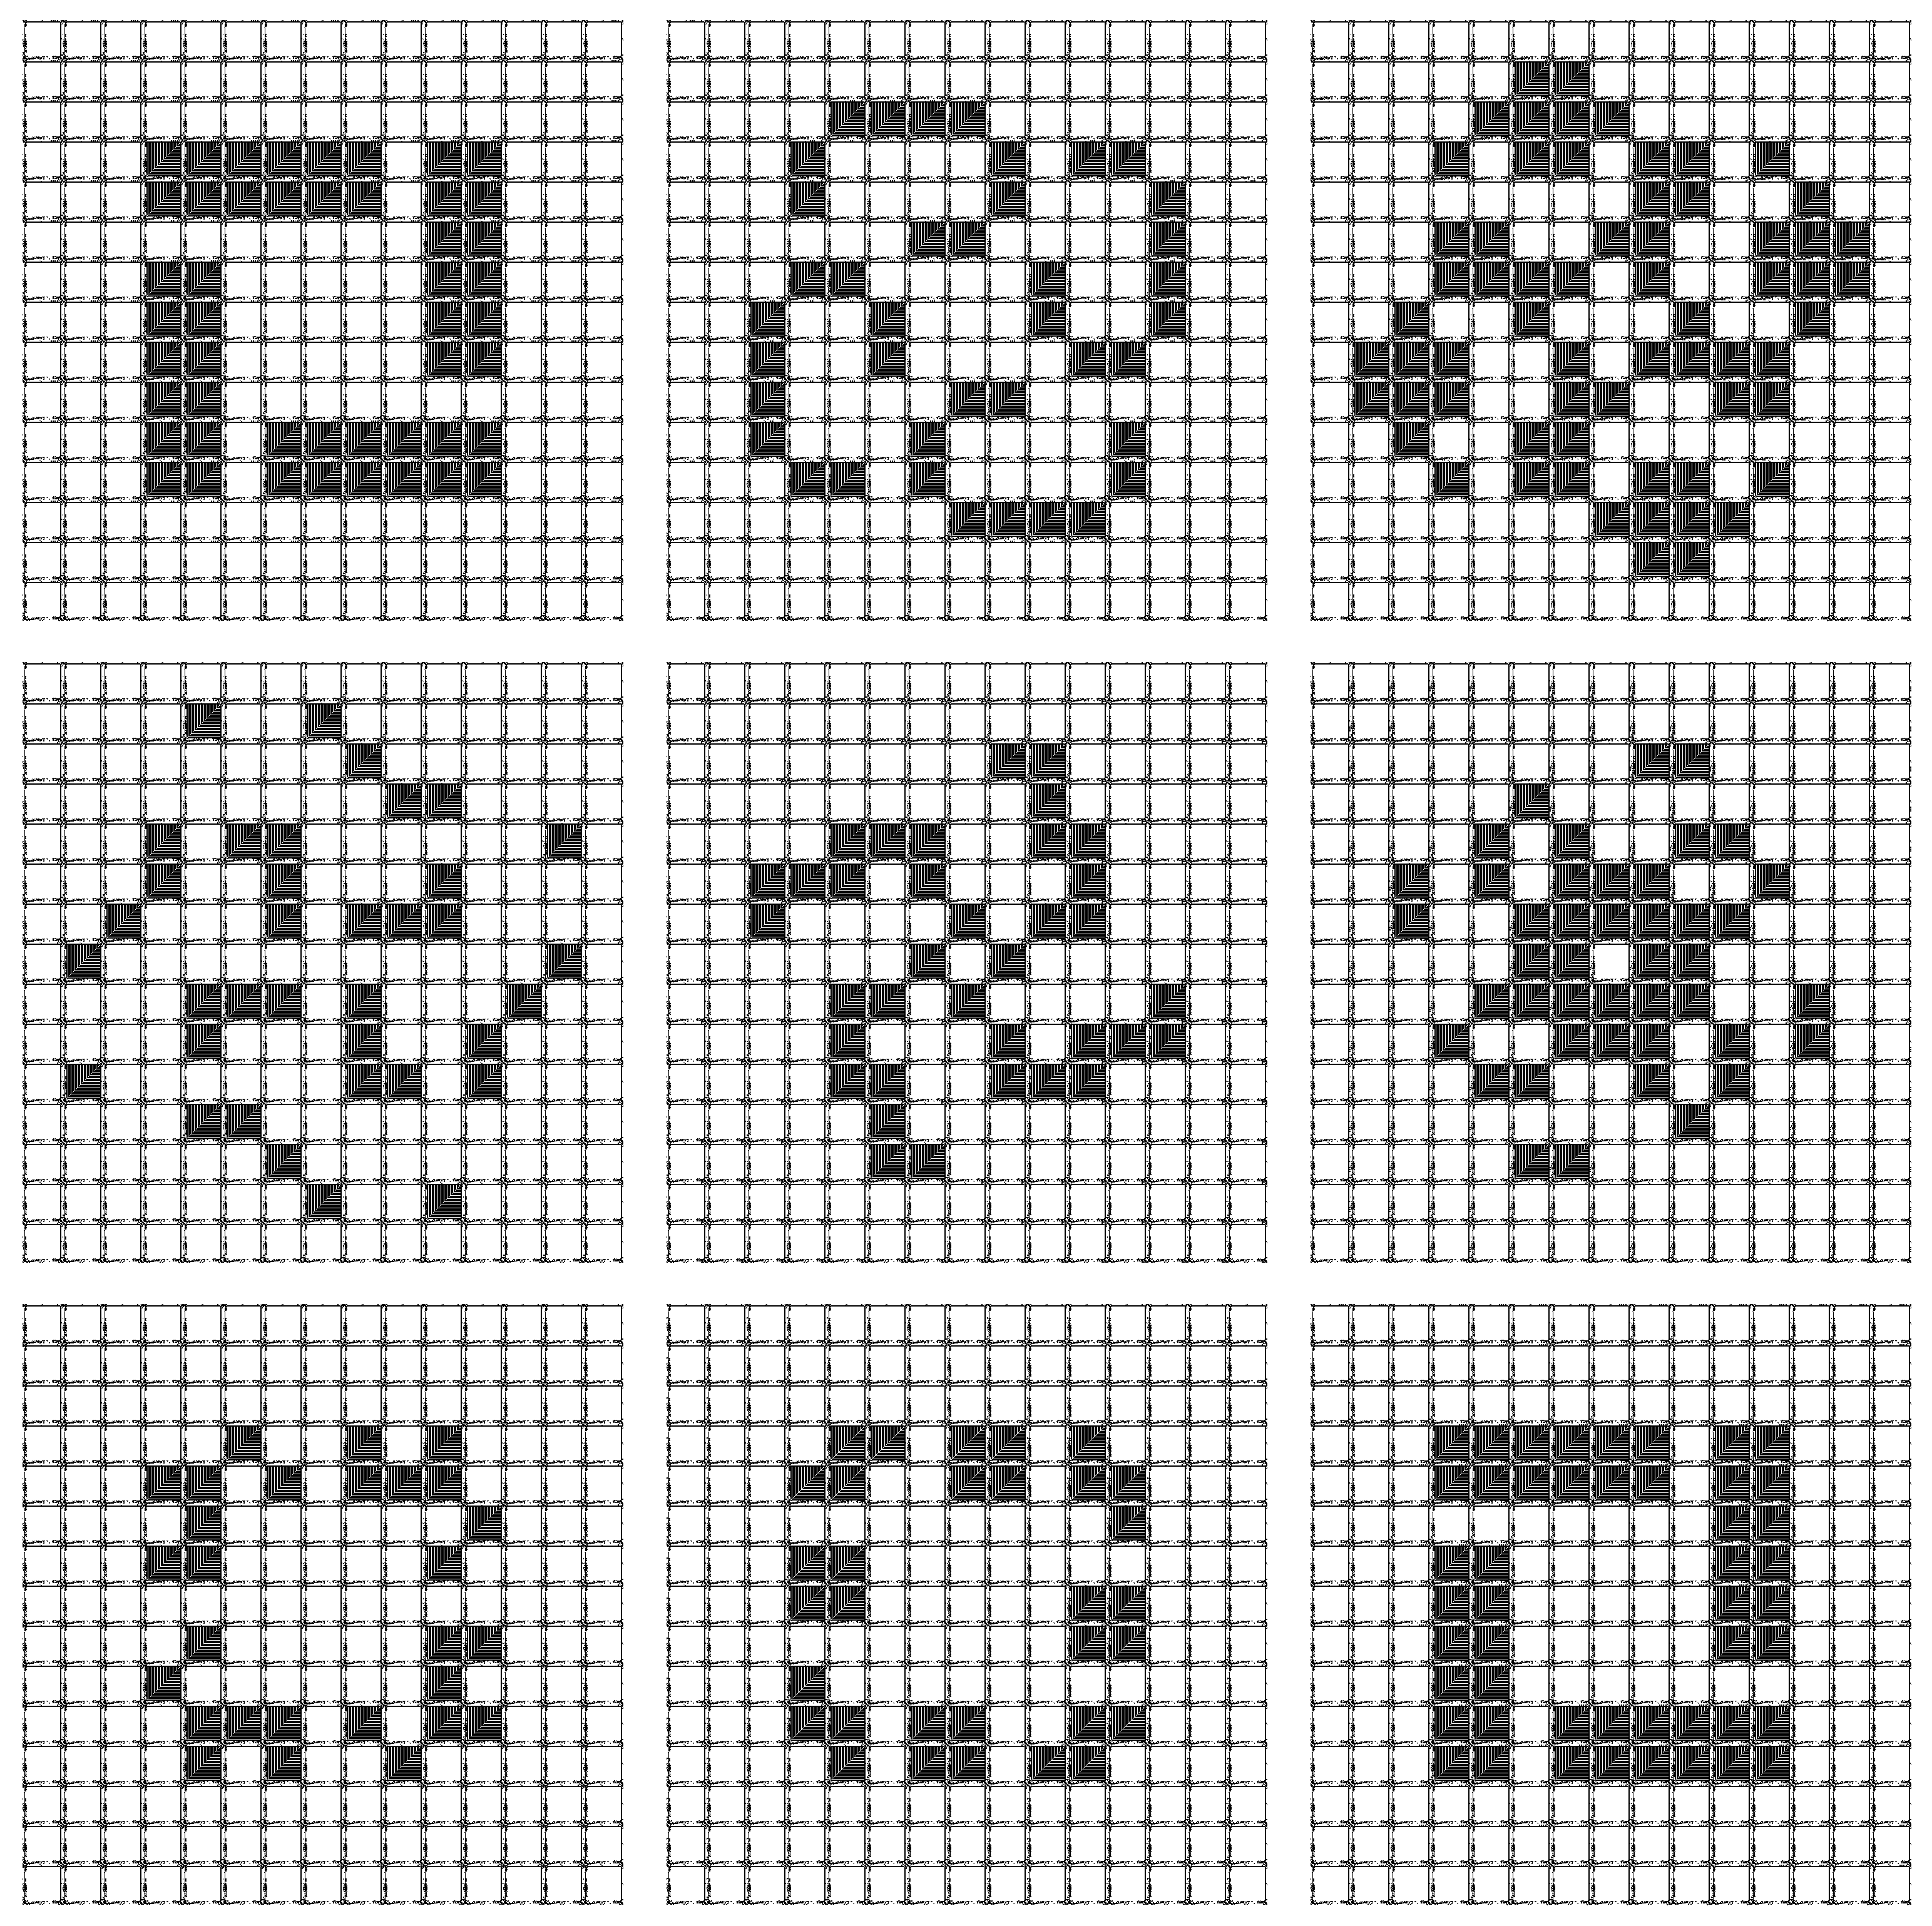
\includegraphics[width=\textwidth]{OTCAGalaxy.png}
  \caption{Nine timesteps of a 15x15 array of OTCA Metapixels playing out a period-8 oscillating pattern called "Kok's Galaxy".  Each time-step represents 35,328 generations of Life; the entire 8 step sequence takes 282,624 generations to complete.  Each metacell occupies 2058x2058 Life cells; the complete 15x15 metapixel array totals 30,800x30,800 Life cells (accounting for a 5 cell overlap between adjacent metacells).  10x magnification of a "living" and "dead" cell are shown at the top of the image.}
  \label{fig:OTCAGalaxy}
\end{figure}

In the next sections, I'll analyze a particularly complex Life pattern in terms of the hierarchies I introduced earlier in the chapter.  The OTCA Metapixel was designed by Brice Due in 2006.  Though not the first \textit{metacell} (a structure that can mimic a CA cell), it is the first \textit{metapixel} (a structure that looks and behaves like a macro-scale CA pixel) built in Life, and it can be programmed to perform any CA ruleset that's based on a summation of a cell's 8 local neighbors.  Many metapixels can be patterned together on a grid to play out a macro-scale CA (Figure \ref{fig:OTCAGalaxy}).  The following analysis is based off of information on Brice Due's website \cite{Due2006} and by watching the pattern run in Golly; I wrote a more detailed discussion of the inner workings of the pattern on Instructables \cite{Ghassaei2015}.\\

\textit{(I chose to analyze this pattern because its square aspect ratio makes it well suited for displaying in a static text like this writeup; known self-replicating patterns do not fit onto one piece of paper at a reasonable scale.)}  

\subsection{Elements, Motifs, and Functions}

\begin{sidewaysfigure}
  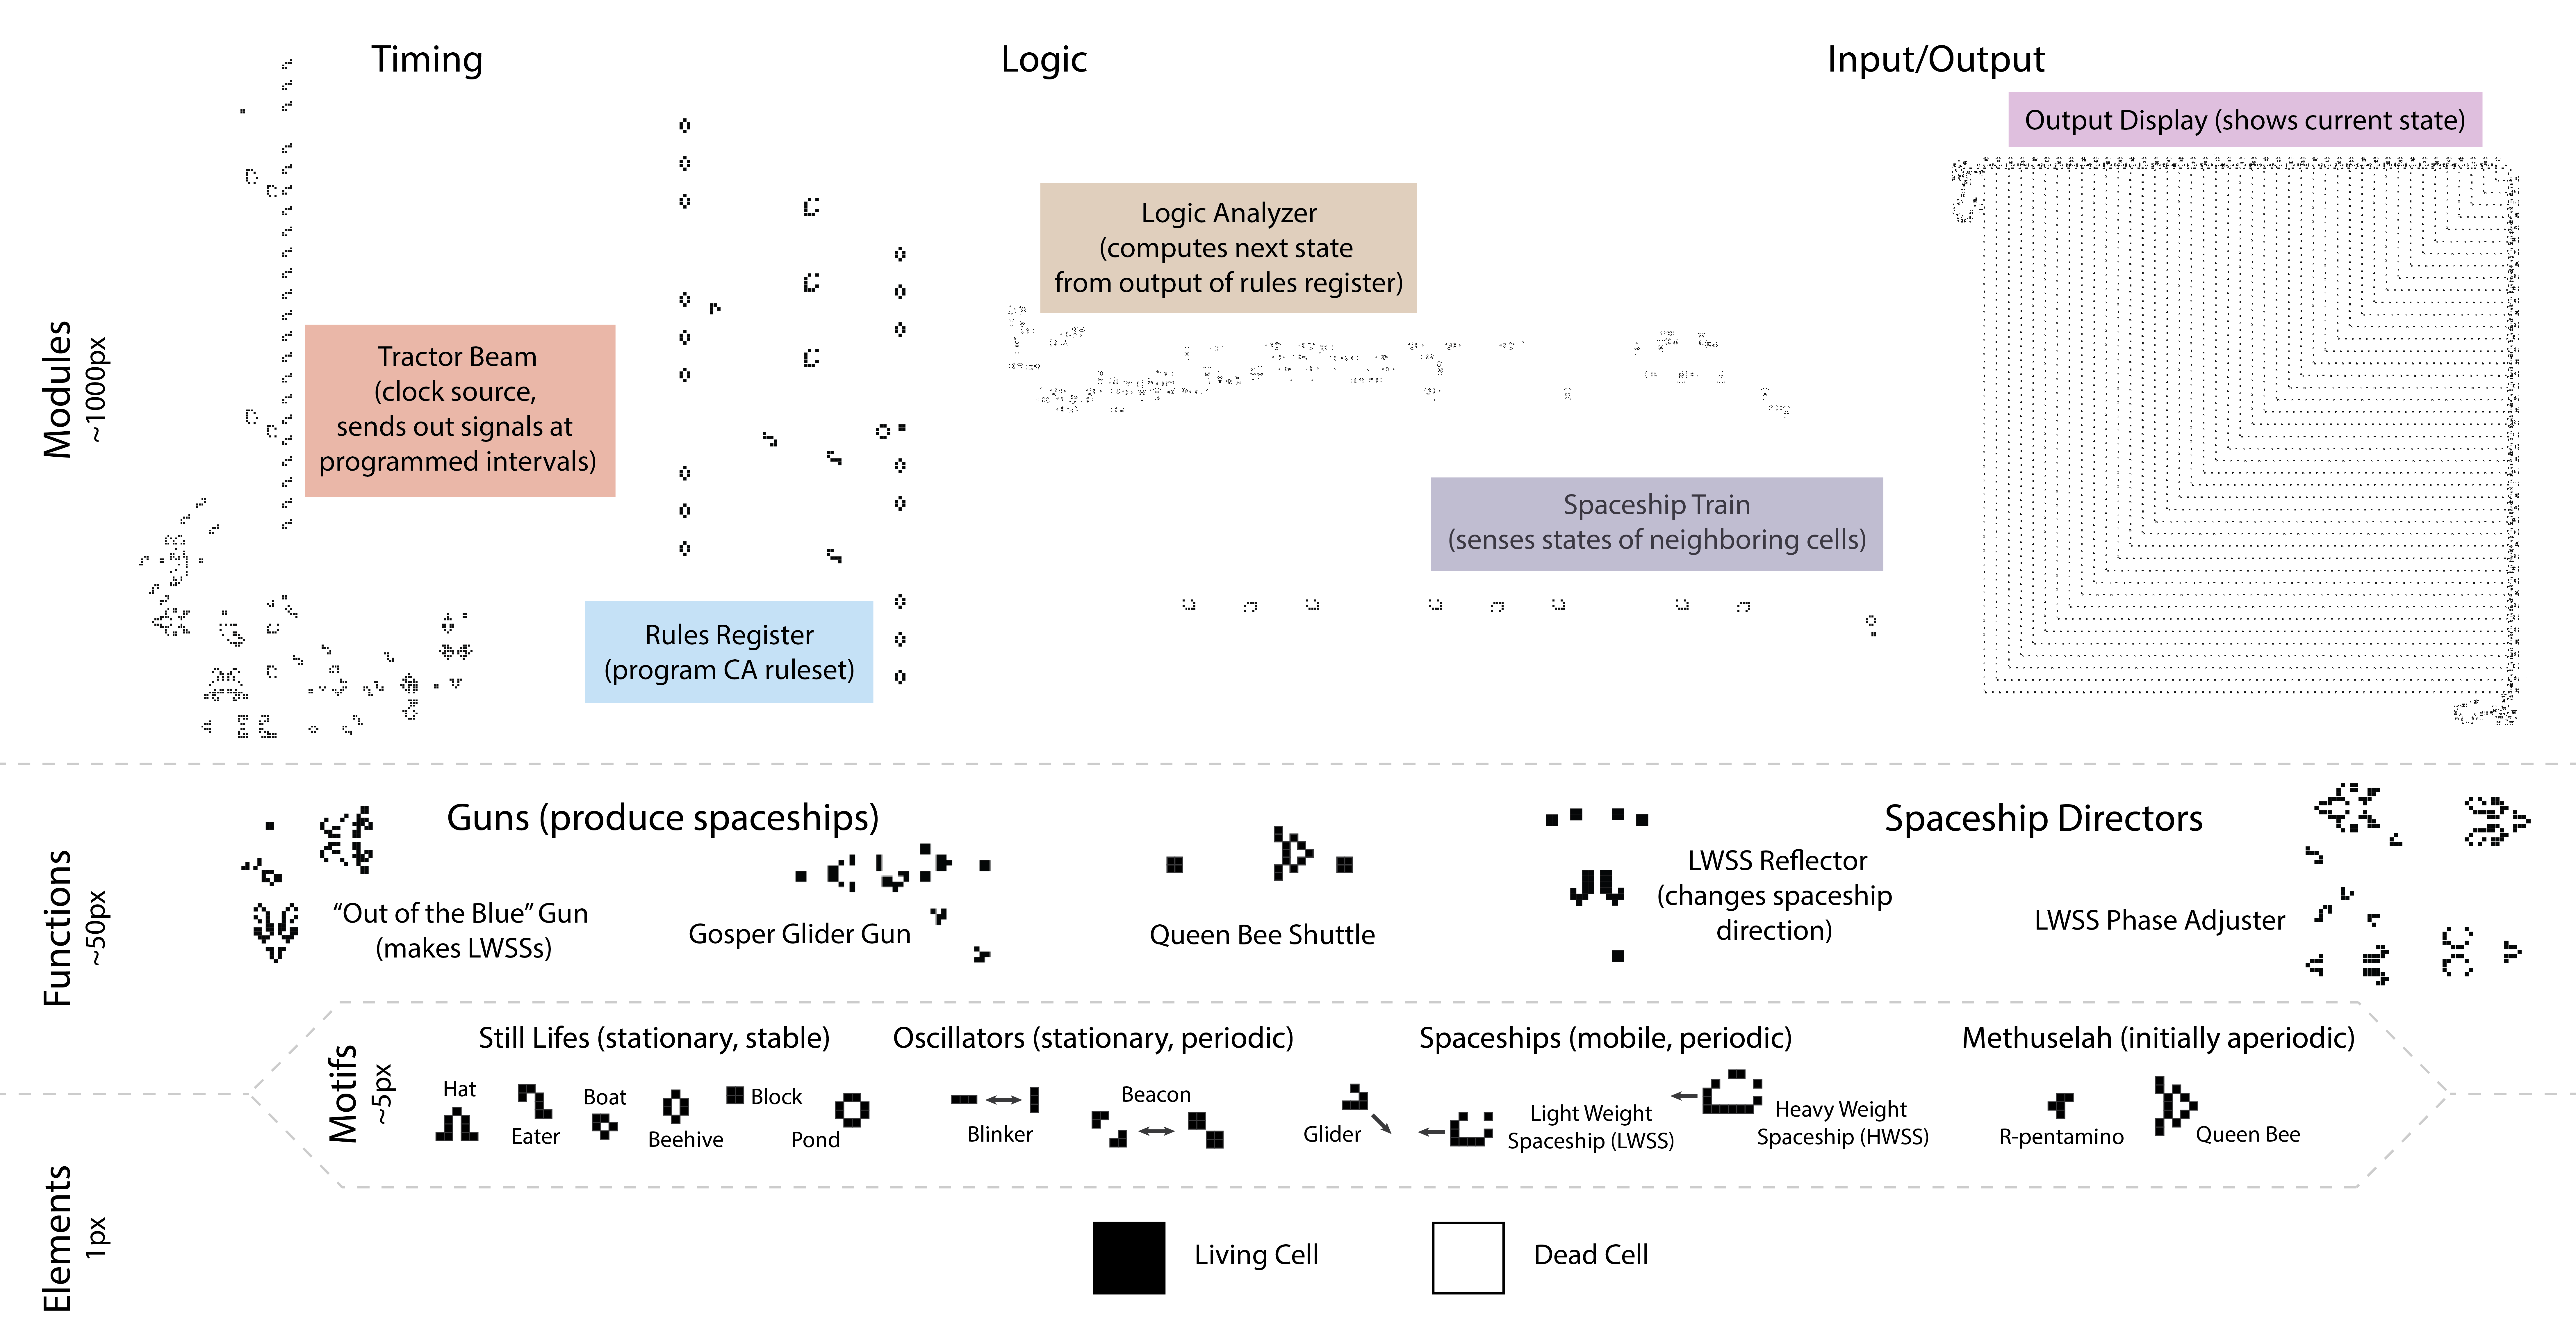
\includegraphics[width=\textwidth,height=\textheight,keepaspectratio]{OTCAMetaHierarchy.png}
  \caption{Hierarchical breakdown of OTCA Metapixel into modules, functions, motifs, and elements.  Complex-level diagram is shown in Figure \ref{fig:OTCADiagram}.}
  \label{fig:OTCAMetaHierarchy}
\end{sidewaysfigure}

The first few levels of hierarchy within Life are illustrated in Figure \ref{fig:OTCAMetaHierarchy}.  At the most basic level, structures within Life are constructed from \textit{cells}.  Each cell is represented by one pixel on a Life grid and stores a binary state - "living" or "dead".  Cells interact with each other according to Conway's rules: living cells with 2 or 3 neighbors stay alive, dead cells with exactly 3 neighbors become living, and all other configurations die or stay dead.  Though the logic of cell-cell interactions is simple, the long term behavior of a given initial condition is difficult to intuit. \\

Small assemblies of cells form \textit{motifs} on the order of about 5 cells across.  \textit{Still Lifes} are a category of motif that are static across time unless acted upon by another pattern.  \textit{Oscillators} repeatedly morph between several conformations at some regular time interval.  Oscillators are categorized based on their period, for example, the Blinker and Beacon are period-2 oscillators, and Kok's Galaxy (Figure \ref{fig:OTCAGalaxy}) is a period-8 oscillator.  \textit{Spaceships} are oscillators that move across the Life grid as they oscillate.  Gliders, the smallest type of spaceship in Life, move across space in diagonal directions.  Other spaceships, such as Light Weight, Medium Weight or Heavy Weight Spaceships (LWSS, MWSS, and HWSS, respectively) move in cartesian directions.  Spaceships are categorized based on their period and on their speed.  \textit{Methuselahs} are small patterns that take a large number of generations to eventually stabilize.  R-Pentamino is a Methuselah of only 5 initial cells that stabilizes in 1103 generations.\\

At the function-level, Life patterns on the scale of about 50 cells interact with each other in more structured and predictable ways.  In order for two function-level patterns to be compatible, they must have compatible periods.  For example, a train of period-4 LWSSes is compatible with a period-46 Twin Bees Shuttle as long the LWSSes in the train are spaced out by 11.5 cycles or some multiple of 11.5 cycles.\\

\textit{Guns} are oscillators that create a train of regularly-spaced spaceships.  Guns are categorized based on the type of spaceships they produce and the frequency at which they produce them.  \textit{Shuttles} are patterns comprised of an active region that oscillates between two stabilizing ends.  Interactions with shuttles can serve a wide variety of functions.  For example, the Twin Bees Shuttle can reflect (change the direction of) gliders, LWSSes, and MWSSes, and it can convert gliders to LWSSes or LWSSes to MWSSes.  The Twin Bees Shuttle forms the basis of the "Out of the Blue" MWSS gun as well as many other period-46 oscillators.  The Queen Bee Shuttle  is made from a Queen Bee that oscillates between two stabilizing blocks.  Two Queen Bee Shuttles form the basis of the Gosper Glider Gun and many other period 30 oscillators.\\

\textit{Reactions} are collisions of Life objects that produce useful outcomes.  The Honeybit reaction is used several times in the OTCA Metapixel to write, store, and read a single bit of data.  In the Honeybit reaction, a glider collides with a Beehive to produce a Pond and a Block - this sets the bit.  Then a LWSS collides with the pond, destroying the LWSS and returning the Pond/Block back to its original Beehive state.  If the bit is not set, the LWSS passes by the beehive unharmed.  \textit{Glider Synthesis} is a process by which complex Life patterns are created solely through the collisions of gliders.  Glider synthesis forms a large subset of known and actively studied Life reactions, and it was a critical piece of Conway's existence proof of a self-replicating universal constructor in Life.  The initial glider configuration pictured in Figure \ref{fig:OTCAMetaHierarchy} is a 6-glider synthesis for the Queen Bee Shuttle; an 8-glider synthesis is known for the Gosper Glider Gun and the Twin Bees Shuttle.\\

A more complete discussion of Life patterns and their history can be found on the Life Wiki \cite{Authors2016} or the Life Lexicon \cite{Silver2016}.

\subsection{Modules and Complexes}

\begin{figure}
  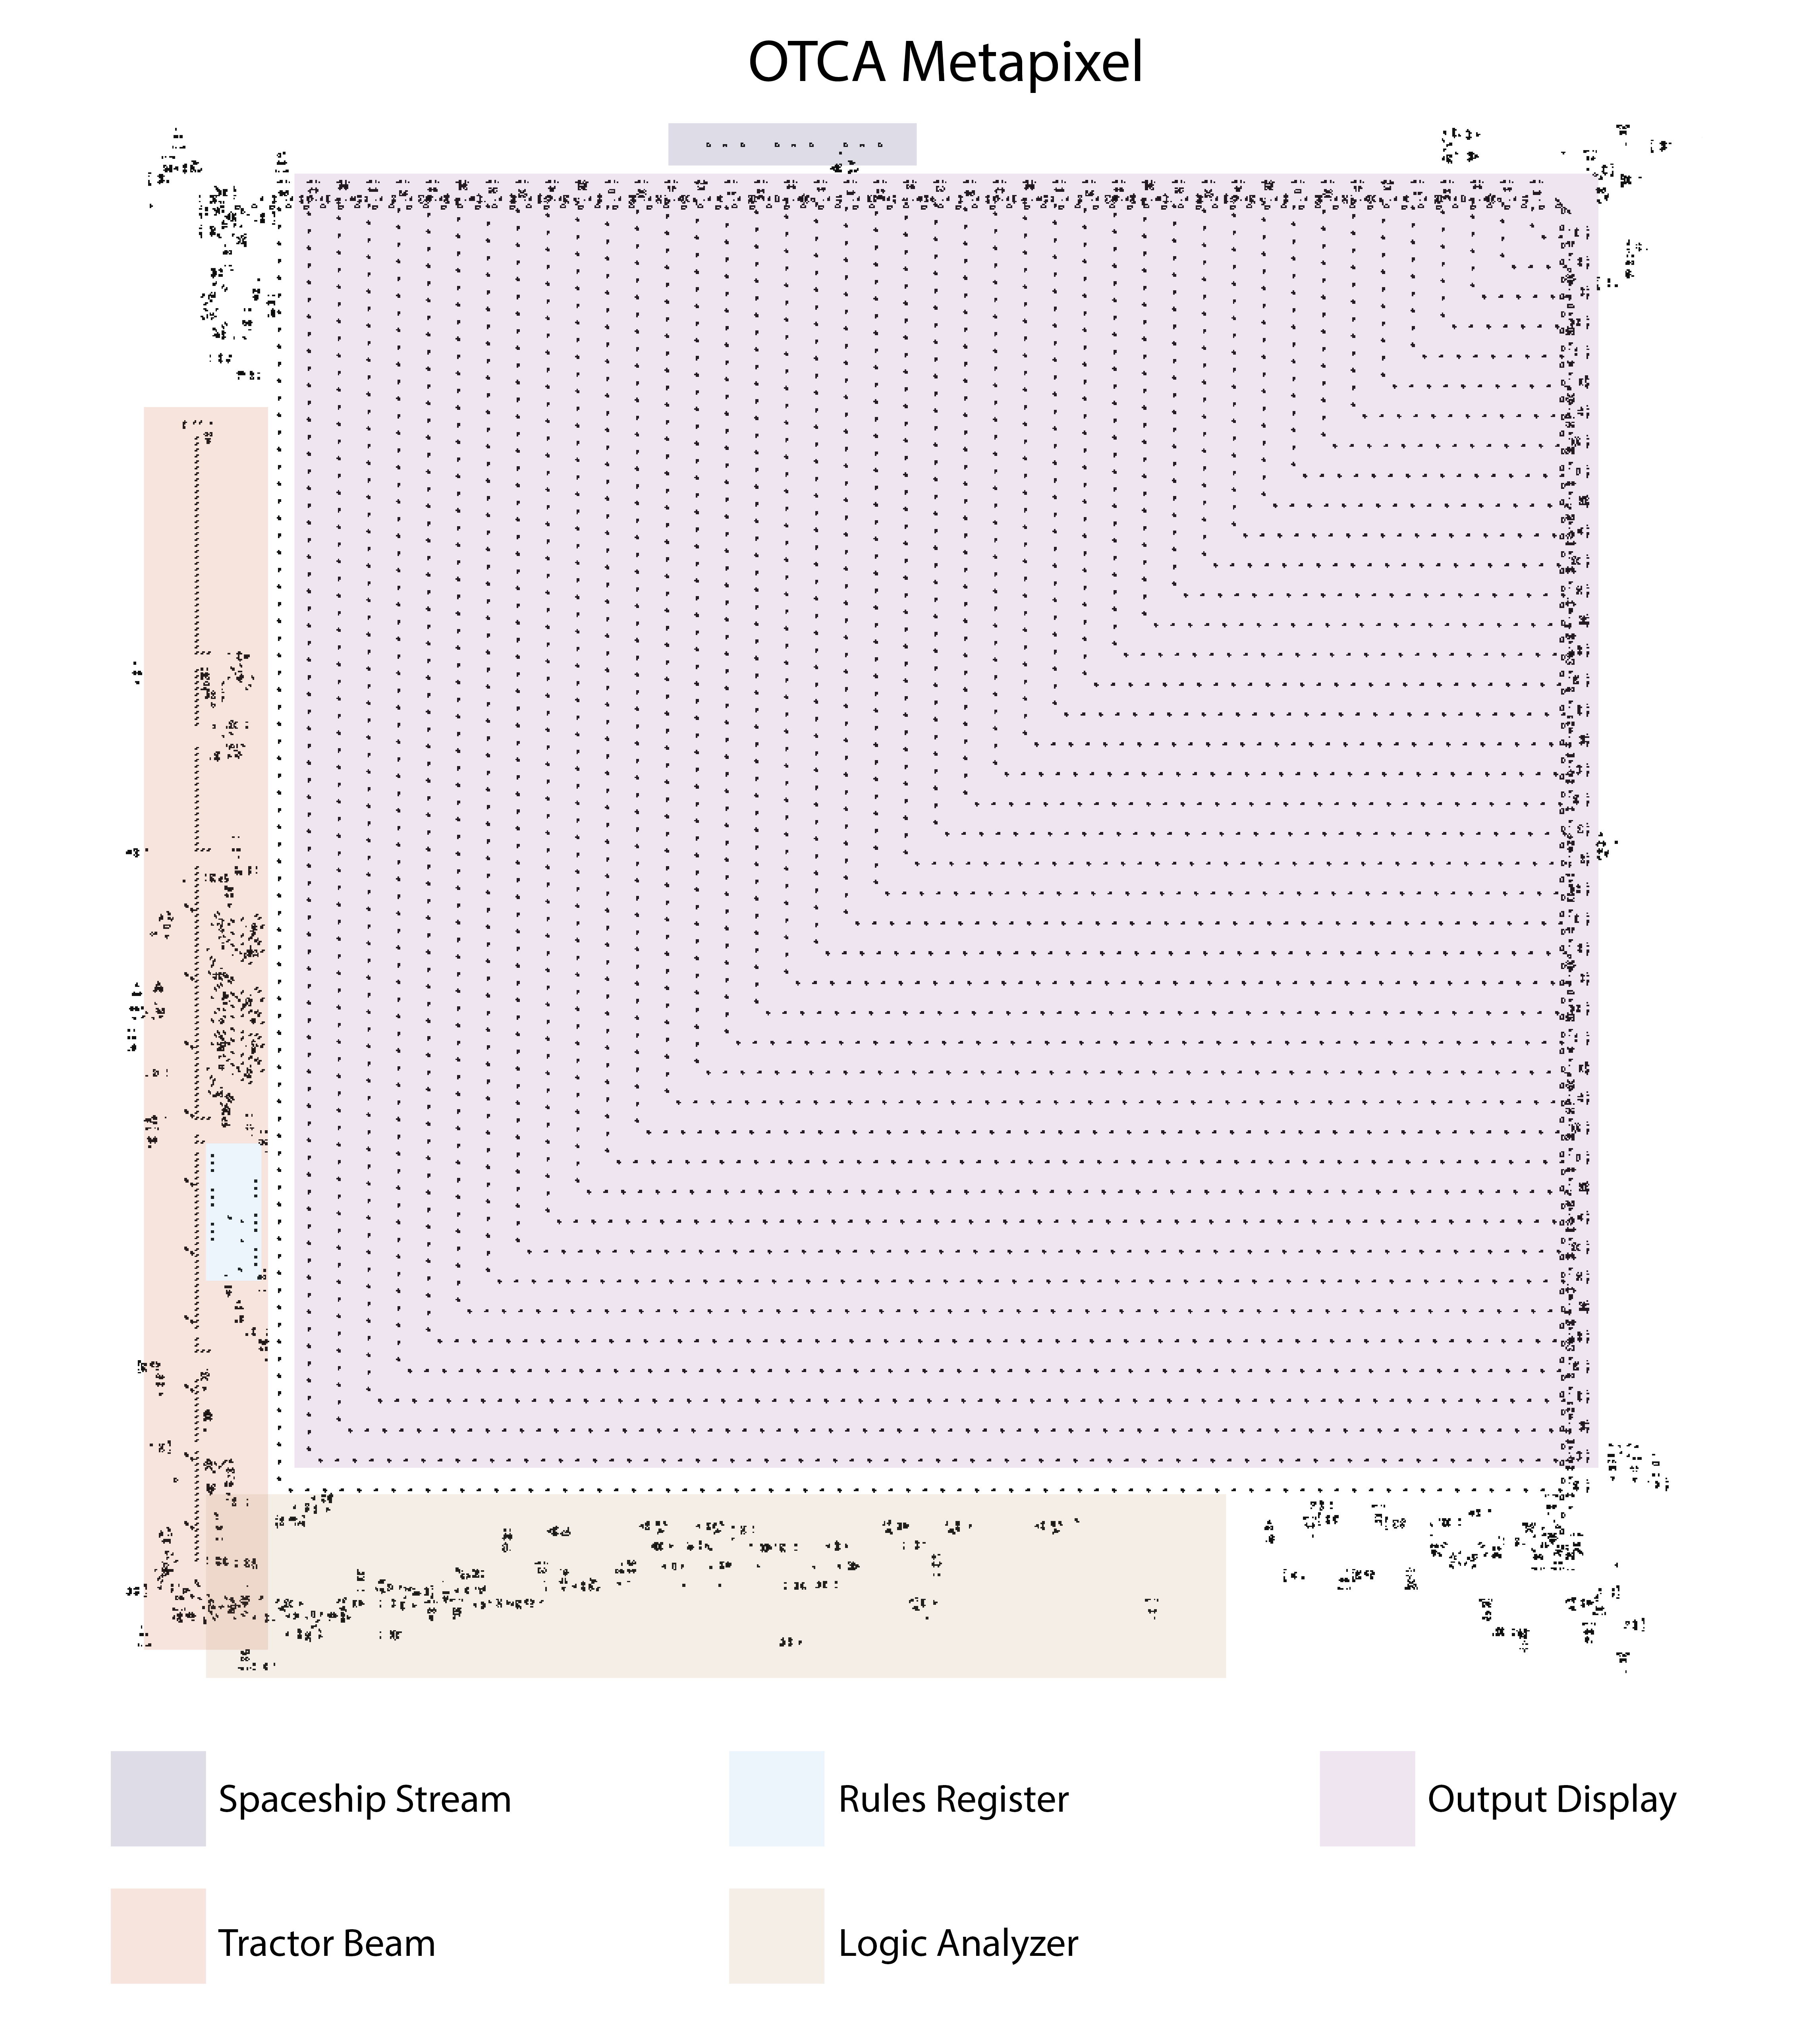
\includegraphics[width=\textwidth]{OTCADiagram.png}
  \caption{Complex-level diagram of OTCA Metapixel with the most important modules highlighted.  Further breakdown of modules into functions, motifs, and elements given in Figure \ref{fig:OTCAMetaHierarchy}.}
  \label{fig:OTCADiagram}
\end{figure}

Modules in Life are designed from functions and motifs to complete a singular, high-level task in a Life machine.  Modules typically range in size from 100 to several thousand cells across.  As with functions, modules must have compatible periods in order to be compatible with one another.  Modules dictate the overall frequency at which a Life machine operates.\\

Spaceship \textit{tapes} are often used to store, move, and execute binary information in Life machines.  These tapes are read through collisions with other objects; the presence or absence of a spaceship in a given position on the tape will dictate the outcome of the collision.  Collisions between two tapes form basic bit-wise logical operations.  Information on the tapes is often duplicated prior to being operated on in order to preserve the original data.  The Spaceship Train (of LWSSes) in the OTCA Metapixel travels in a loop around the perimeter of the cell, collecting a tally of the neighboring states through collisions with Honeybits.  The components of this module include the train itself, the reflectors and other modifiers used to direct the train along its course, and the Honeybit reactions set by neighboring cells.\\

Machines often require a central \textit{events timer} to trigger the start and stop of key tasks.  A Tractor Beam clock is typically used for this purpose in Life.  Tractors beams are a type of gun aimed at a still life, such that each collision between the tractor beam's spaceship stream and the still life moves the still life some increment closer to the tractor beam's source.  In a sense a tractor beam "pulls" the still life toward it.  When the still life reaches some critical distance to the tractor beam source, it is destroyed and re-synthesized in its original starting position.  The time it takes for the still life to complete one cycle of this behavior determines the overall period of the tractor beam clock; this period is programmed by controlling the initial distance of the still life from the tractor beam.  The OTCA Metapixel's events timer shoots a stream of LWSSes and MWSSes towards a Block, moving the Block down by 8 cells in each collision; a complete cycle of the events timer takes 35,328 generations.  The events timer has an added feature that a glider is ejected to the right during each collision with the Block.  A fence of Eaters typically annihilates the glider immediately, but programmed holes in the fence allow the glider to pass through and trigger events at arbitrary phases of one complete cycle.\\

The OTCA Metapixel \textit{displays its current state} by toggling on and off two banks of MWSS guns, whose streams intersect and mutually annihilate each other in the center of the pattern.  Each bank is controlled by a simple latching mechanism, which toggles a LWSS gun on and off.  When this gun is on, it interacts with a bank of shuttles in an "Out of the Blue" reaction, effectively turning them into MWSS guns.\\

A rules \textit{register} is a type of persistent memory that is used, in the case of the OTCA Metapixel, to encode the rules of a CA.  Inside the register, a collision with the Spaceship Train and a Honeybit reaction compare the number of living neighbors with the rules stored in the register.  The OTCA metapixel's register capacity tops off at 16 bits of information.  In order to store arbitrarily large numbers in this type of register or on one of the tapes described above, the register/tape would need to be infinite.  Marvin Minsky described a type of finite-sized memory register with infinite memory capacity that solves this problem in 1967 \cite{Minsky1967}.  Dean Hickerson designed the Minsky register in Life \cite{Hickerson1900} in 1990 based on a description given by Conway in Winning Ways \cite{Berekamp1982}.  This paved the way for the development of a universal computer with finite size, built by Paul Chapman in 2002 \cite{Chapman2002}.\\

A static \textit{logic bank} is constructed within a machine to interpret data, typically from incoming spaceship tapes.  Simple bitwise logical operators (not, and, or, nor, etc) can be computed on one or more pieces of data.  The output from the OTCA Metapixel's rules register is fed into a logic bank in order to determine the next state of the metacell.

\subsection{Insights}

The previous sections illustrates design hierarchy in one example of a complex, programmable Life machine.  Moving from elemental cells, to motifs and functions, to modules, and finally to complexes introduces scaling on the order of 10-50x at each level.  As with biological systems, function and motif-level structures are highly reusable in the design of module-level objects.  Modules tend to be more highly tuned to the specific needs of the larger complex they belong to, both in terms of their time-dependencies and geometric layout; in general this means a module may need some editing to work within a complex it was not originally designed for.

\subsubsection{Design}

Human-directed design in Life occurs at the level of motif and function-level building blocks, based on a knowledge of codified interactions between them.  It is entirely possible that a seemingly random assortment of Life cells produce desired high-level behaviors such as programmable self-replication.  However, it would not be possible for a human to design a complex machine in Life by placing elemental parts without some notion of hierarchical abstraction.  As with functional groups in organic chemistry, motifs and functions in Life provide a useful abstraction from the low level physics of the system.  Without this abstraction, it is nearly impossible to develop an intuition about how a complex Life pattern will behave.  Furthermore, it is likely that we would recognize familiar motifs within any complex Life pattern, human-designed or not.  Small still lifes, oscillators, and spaceships spontaneously arise from random initial conditions with high frequency \cite{Flammenkamp2004}.

\subsubsection{Evolutionary Potential}

Interactions between a Life machine and debris in the environment could edit spaceship tapes, change logical outcomes, or affect other programmed functions of the machine.  Some of these interactions could result in permanent changes to the functioning of the machine.  As with genetic mutations in coding regions of the genome, most changes to the machine's inner workings would be deleterious to the overall functioning of the machine, however, some changes could eventually endow it with new behaviors.

}
